\documentclass[11pt]{article}

% ----------------- Codificação e Idioma -----------------
\usepackage[utf8]{inputenc}
\usepackage[T1]{fontenc}
\usepackage[brazilian]{babel}

% ----------------- Pacotes Essenciais e Gráficos -----------------
\usepackage{amsmath, amsfonts, amssymb, amsthm}
\usepackage{float}
\usepackage{booktabs}
\usepackage{caption}
\usepackage{xcolor}
\usepackage{tcolorbox}
\usepackage{graphicx}
\usepackage{url}
\usepackage[a4paper, margin=2.5cm]{geometry} 
\usepackage{listings}

\usepackage{amsmath}
\DeclareMathOperator{\Var}{Var}

% ----------------- Pacote e configuração para gerenciar as definições -----------------
\theoremstyle{definition} 
\newtheorem{definicao}{Definição}
\newtheorem{teorema}{Teorema}
\newtheorem{corolario}{Corolário}
\newtheorem{axioma}{Axioma}
\newtheorem{exemplo}{Exemplo}


% ----------------- Formatação de Parágrafos -----------------
\usepackage{indentfirst}
\setlength{\parindent}{1.25cm} 
\setlength{\parskip}{0.2cm}    


% ----------------- Hyperref e Bibliografia (Ordem Importante) -----------------
% O hyperref precisa ser carregado ANTES do backref e do abntex2cite
\usepackage{hyperref} 
\usepackage[brazilian,hyperpageref]{backref}     % Paginas com as citações na bibl
\usepackage[alf]{abntex2cite}                    % Citações padrão ABNT

% ----------------- Cores e Estilo para Código (Ex: R) -----------------
\definecolor{gray}{rgb}{0.5,0.5,0.5}
\definecolor{lightgray}{rgb}{0.95,0.95,0.95}
\definecolor{mygreen}{rgb}{0,0.6,0}
\definecolor{myblue}{rgb}{0,0,0.8}
\hypersetup{hidelinks}

\lstset{
	language=R,
	backgroundcolor=\color{lightgray},
	basicstyle=\ttfamily\small,
	keywordstyle=\color{myblue}\bfseries,
	commentstyle=\color{mygreen},
	stringstyle=\color{gray},
	numbers=left,
	numberstyle=\tiny\color{gray},
	stepnumber=1,
	numbersep=5pt,
	showspaces=false,
	showstringspaces=false,
	showtabs=false,
	frame=single,
	breaklines=true,
	tabsize=2,
	inputencoding=utf8,
	extendedchars=true,
	literate=
	{á}{{\'a}}1 {é}{{\'e}}1 {í}{{\'i}}1 {ó}{{\'o}}1 {ú}{{\'u}}1
	{Á}{{\'A}}1 {É}{{\'E}}1 {Í}{{\'I}}1 {Ó}{{\'O}}1 {Ú}{{\'U}}1
	{à}{{\`a}}1 {è}{{\`e}}1 {ì}{{\`i}}1 {ò}{{\`o}}1 {ù}{{\`u}}1
	{À}{{\`A}}1 {È}{{\'E}}1 {Ì}{{\`I}}1 {Ò}{{\`O}}1 {Ù}{{\`U}}1
	{ä}{{\"a}}1 {ë}{{\"e}}1 {ï}{{\"i}}1 {ö}{{\"o}}1 {ü}{{\"u}}1
	{Ä}{{\"A}}1 {Ë}{{\"E}}1 {Ï}{{\"I}}1 {Ö}{{\"O}}1 {Ü}{{\"U}}1
	{â}{{\^a}}1 {ê}{{\^e}}1 {î}{{\^i}}1 {ô}{{\^o}}1 {û}{{\^u}}1
	{Â}{{\^A}}1 {Ê}{{\^E}}1 {Î}{{\^I}}1 {Ô}{{\^O}}1 {Û}{{\^U}}1
	{ã}{{\~a}}1 {ẽ}{{\~e}}1 {ĩ}{{\~i}}1 {õ}{{\~o}}1 {ũ}{{\~u}}1
	{Ã}{{\~A}}1 {Ẽ}{{\~E}}1 {Ĩ}{{\~I}}1 {Õ}{{\~O}}1 {Ũ}{{\~U}}1
	{ç}{{\c{c}}}1 {Ç}{{\c{C}}}1
}

% ----------------- Informações do Documento -----------------
\title{\textbf{Relatório de Atividades}}
\author{Arthur Vitola, Henrique Prange, Kauan Moura, Marcos Silva\\
	Programa de Pós-Graduação em Ciência da Computação\\
	CCET - Unioeste}
\date{\today}

\begin{document}
	
	\maketitle
	\tableofcontents
	\newpage
	
	% ================================================================================
	\section{Introdução}

A incerteza é um elemento inerente a muitos fenômenos estudados na Ciência da
Computação, desde o tempo de resposta de um servidor até o resultado de um
classificador automático. A teoria da probabilidade oferece a linguagem formal
para descrever esses fenômenos e raciocinar sobre eles de maneira quantitativa,
tendo se tornado indispensável na Computação \cite{harcholbalter2024probability}.
Sua base axiomática moderna foi estabelecida por Andrey Kolmogorov em 1933
\cite{kolmogorov1933grundbegriffe}. Na engenharia, a mesma teoria fundamenta a
metodologia estatística empregada na resolução de problemas reais
\cite{montgomery2018applied}.

Boa parte da Computação atual gira em torno de dados, que são inseparáveis da
probabilidade \cite{chan2021probability}. A estatística reúne os métodos de coleta,
análise e interpretação de dados que permitem extrair informação e apoiar decisões
\cite{sahu2024probability}, de modo que estatística e computação se consolidam como
recursos fundamentais na pesquisa e na indústria \cite{ferreira2020estatistica}.
Conceitos como esperança, variância, independência e o Teorema de Bayes aparecem de
forma recorrente em problemas de classificação, diagnóstico e avaliação de
desempenho.

Nem sempre as probabilidades de interesse podem ser obtidas por via puramente
analítica, e a simulação computacional surge como alternativa para estimá-las pela
repetição de um experimento aleatório. Essa abordagem é amplamente usada na
avaliação do desempenho de sistemas computacionais
\cite{harcholbalter2024probability} e tem respaldo na Lei dos Grandes Números, que
garante a convergência das frequências observadas para as probabilidades teóricas
\cite{ross2010probabilidade}. As simulações deste trabalho foram conduzidas em R,
uma linguagem e ambiente para computação estatística e gráfica
\cite{ferreira2020estatistica}, bastante usado para ilustrar conceitos de
probabilidade como o próprio Teorema Central do Limite \cite{sahu2024probability}.
Em todos os experimentos foi fixada a semente do gerador de números aleatórios, o
que assegura a reprodutibilidade dos resultados.

O objetivo deste relatório é revisitar conceitos centrais da probabilidade
combinando o tratamento teórico com experimentos computacionais em R, de modo que
cada propriedade enunciada seja também verificada de forma empírica. O texto está
organizado em torno desses dois eixos, o teórico e o computacional. A primeira
parte trata da simulação de experimentos aleatórios simples, como o lançamento de
uma moeda, a retirada de bolas de uma urna e a soma de dois dados, e introduz a
frequência relativa como estimador de probabilidade. Em seguida são estudadas as
distribuições discretas e as distribuições contínuas, com destaque para o Teorema
Central do Limite, que descreve a aproximação da média amostral à distribuição
normal. A esperança e a variância são então analisadas em conjunto com a Lei dos
Grandes Números, que formaliza a estabilidade das médias amostrais. A parte
seguinte aborda a probabilidade condicional, a independência de eventos e o Teorema
de Bayes, aplicados a problemas como filtragem de spam, diagnóstico médico e
autenticação biométrica. Por fim, uma atividade integradora final reúne vários
estudos que aplicam e combinam os conceitos anteriores em problemas de inspiração
computacional, alguns deles apoiados em modelos clássicos da probabilidade aplicada
\cite{ross2024models}.

	
	\section{Simulação de Experimentos Aleatórios em R}

A simulação computacional permite reproduzir experimentos aleatórios cujo
resultado não pode ser previsto com certeza. Na Ciência da Computação, em que a
probabilidade é indispensável, a simulação é um recurso importante na avaliação
do desempenho de sistemas \cite{harcholbalter2024probability} e também no
tratamento de problemas em que os dados dependem de um modelo
probabilístico \cite{chan2021probability}. Nesta seção, as funções
\textit{runif()}, \textit{sample()} e \textit{replicate()} são usadas para simular,
respectivamente, uma moeda, uma urna e a soma de dois dados, comparando as
frequências empíricas com as probabilidades teóricas. Ao final, a soma de dois
dados também ilustra a convergência da média amostral à medida que o número de
repetições aumenta.

A frequência relativa de um evento $A$, observado em $n$ repetições de um
experimento aleatório, é definida como a razão apresentada na
Equação~\ref{eq:freq}.

\begin{equation}
	f_n(A) = \frac{n_A}{n}
	\label{eq:freq}
\end{equation}

Na Equação~\ref{eq:freq}, $n_A$ conta quantas vezes o evento $A$ ocorreu nas $n$
repetições. Sob a interpretação frequentista, a probabilidade teórica $P(A)$
corresponde ao valor para o qual a frequência relativa converge quando o número
de repetições cresce, o que se denota por
$P(A) = \lim_{n \to \infty} f_n(A)$. Esse comportamento é garantido pela Lei dos
Grandes Números e é o que permite estimar
probabilidades por meio de simulação \cite{ross2010probabilidade}.

\subsection{Moeda e a convergência da frequência relativa}

Para simular uma moeda honesta, foram gerados $n = 5000$ números aleatórios
uniformes em $[0,1]$ com a função \textit{runif()}, contando como ``cara'' cada
valor menor que $0{,}5$. Como a probabilidade de um número uniforme cair abaixo de
$0{,}5$ é exatamente $0{,}5$, esse procedimento reproduz uma moeda honesta com
$P(\text{cara}) = 0{,}5$. Cada lançamento equivale a uma variável aleatória de
Bernoulli $X_i$, que assume o valor $1$ para cara e $0$ caso contrário. Como $X_i$
é uma variável indicadora e os lançamentos são independentes e identicamente
distribuídos \cite{harcholbalter2024probability}, a frequência relativa de caras
após $n$ lançamentos coincide com a média amostral dessas variáveis, definida na
Equação~\ref{eq:media_bernoulli}.

\begin{equation}
	\bar{X}_n = \frac{1}{n} \sum_{i=1}^{n} X_i
	\label{eq:media_bernoulli}
\end{equation}

Pela Lei dos Grandes Números, a média amostral $\bar{X}_n$ converge para o valor
esperado $E[X_i] = p = 0{,}5$ quando $n$ cresce \cite{ross2010probabilidade}. O
Listing~\ref{lst:moeda} gera os números uniformes e acompanha a frequência
relativa acumulada de cara.

\begin{lstlisting}[caption={Moeda simulada com \textit{runif()} e frequência relativa acumulada.}, label={lst:moeda}]
n_moeda <- 5000
result <- runif(n_moeda)
eh_cara <- result < 0.5
freq_rel <- cumsum(eh_cara) / seq_len(n_moeda)
\end{lstlisting}

A convergência dessa frequência aparece na Figura~\ref{fig:moeda}. Apesar da
forte oscilação inicial, a frequência relativa se estabiliza em torno do valor
teórico $0{,}5$ conforme $n$ cresce. A frequência relativa final observada foi
$0{,}4948$, com desvio de $0{,}0052$ em relação ao valor teórico.

\begin{figure}[H]
	\centering
	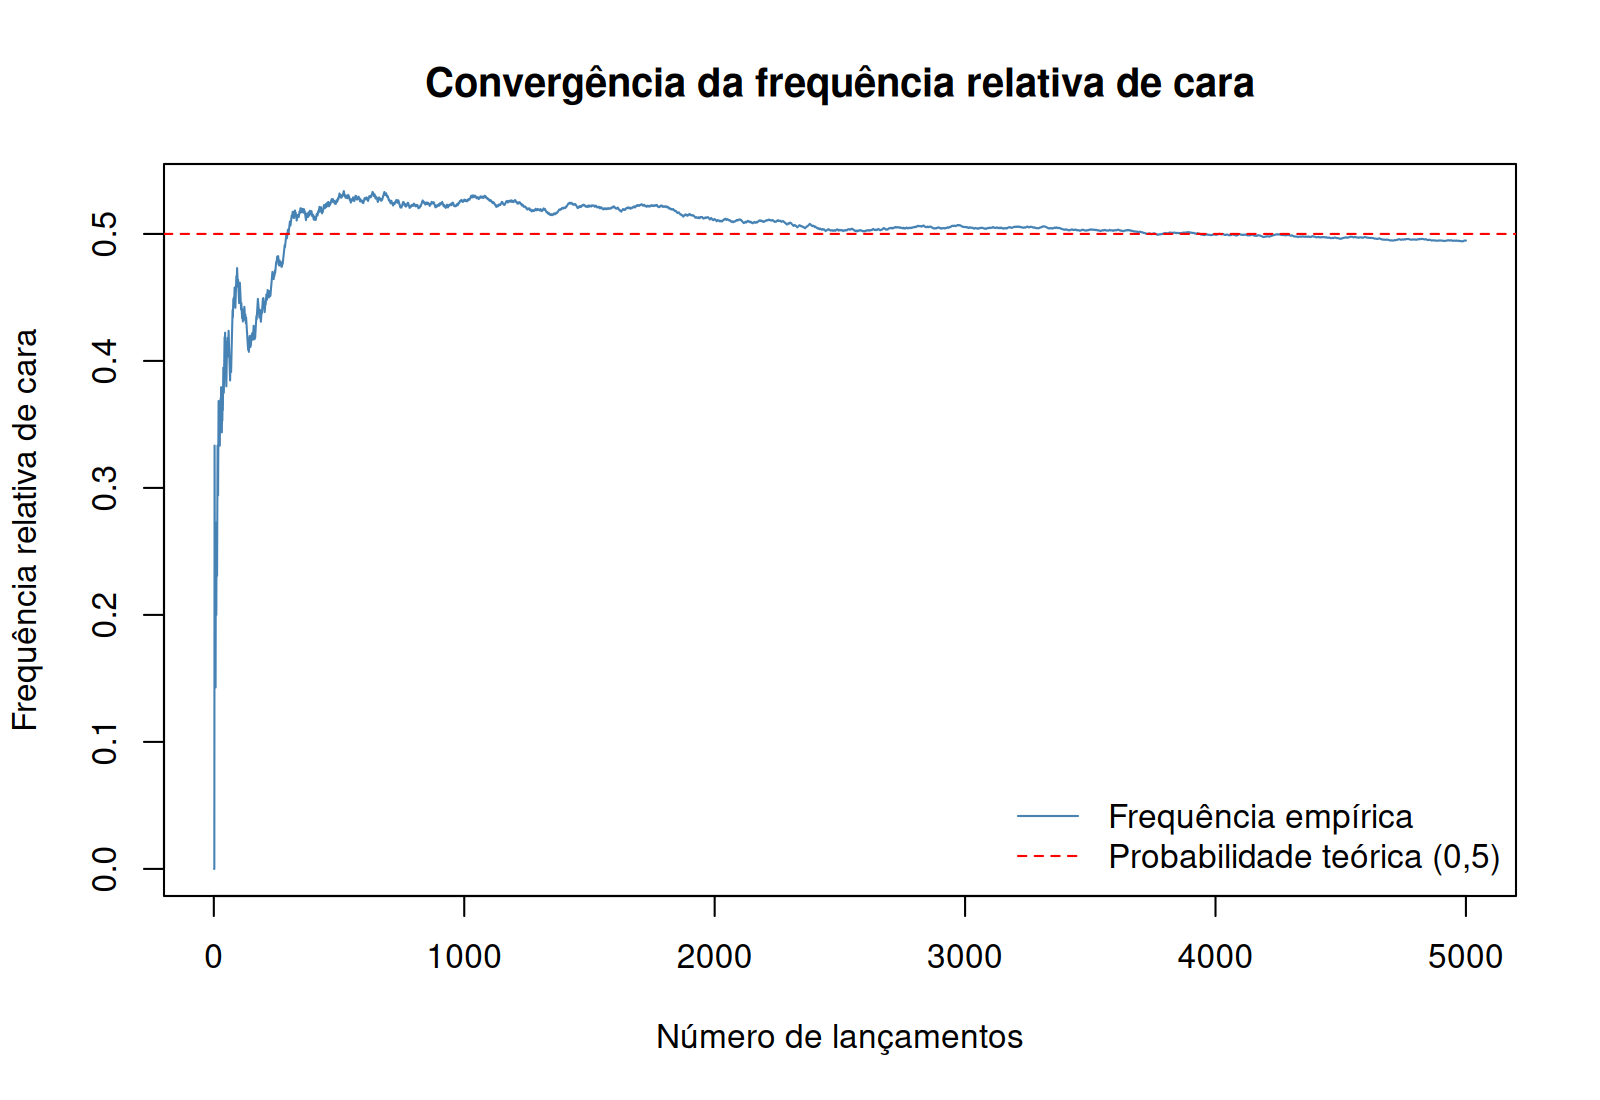
\includegraphics[width=0.8\textwidth]{secoes/02_simulacao/imagens/fig_moeda_convergencia.png}
	\caption{Convergência da frequência relativa de ``cara'' para $0{,}5$.}
	\label{fig:moeda}
\end{figure}

\subsection{Urna e a amostragem aleatória}

É considerada uma urna com 10 bolas, sendo 5 vermelhas, 3 azuis e 2 verdes. A
probabilidade de retirar uma bola de determinada cor é obtida pela razão entre o
número de bolas daquela cor e o total de bolas na urna, conforme a
Equação~\ref{eq:prob_urna}.

\begin{equation}
	P(\text{cor}) = \frac{\text{número de bolas da cor}}{\text{número total de bolas}}
	\label{eq:prob_urna}
\end{equation}

Pela Equação~\ref{eq:prob_urna}, as probabilidades teóricas de retirar cada cor
são, respectivamente, $5/10 = 0{,}5$, $3/10 = 0{,}3$ e $2/10 = 0{,}2$. Como cada
retirada é feita com reposição, o experimento é repetido sob condições idênticas
e de forma independente, de modo que as frequências relativas observadas estimam
as probabilidades teóricas \cite{ross2010probabilidade}. O Listing~\ref{lst:urna}
sorteia $n = 8000$ retiradas com a função \textit{sample()}.

\begin{lstlisting}[caption={Retiradas de uma urna com \textit{sample()}.}, label={lst:urna}]
urna <- c(rep("vermelha", 5), rep("azul", 3), rep("verde", 2))
n_urna <- 8000
retiradas <- sample(urna, size = n_urna, replace = TRUE)

freq_emp_urna <- table(factor(retiradas, levels = c("vermelha", "azul", "verde"))) / n_urna
prob_teo_urna <- c(0.5, 0.3, 0.2)
\end{lstlisting}

Os resultados aparecem na Figura~\ref{fig:urna}. As frequências observadas foram
$0{,}4984$ para vermelha, $0{,}2940$ para azul e $0{,}2076$ para verde, próximas
da composição real da urna, com desvio máximo de cerca de $0{,}008$ em relação
aos valores teóricos.

\begin{figure}[H]
	\centering
	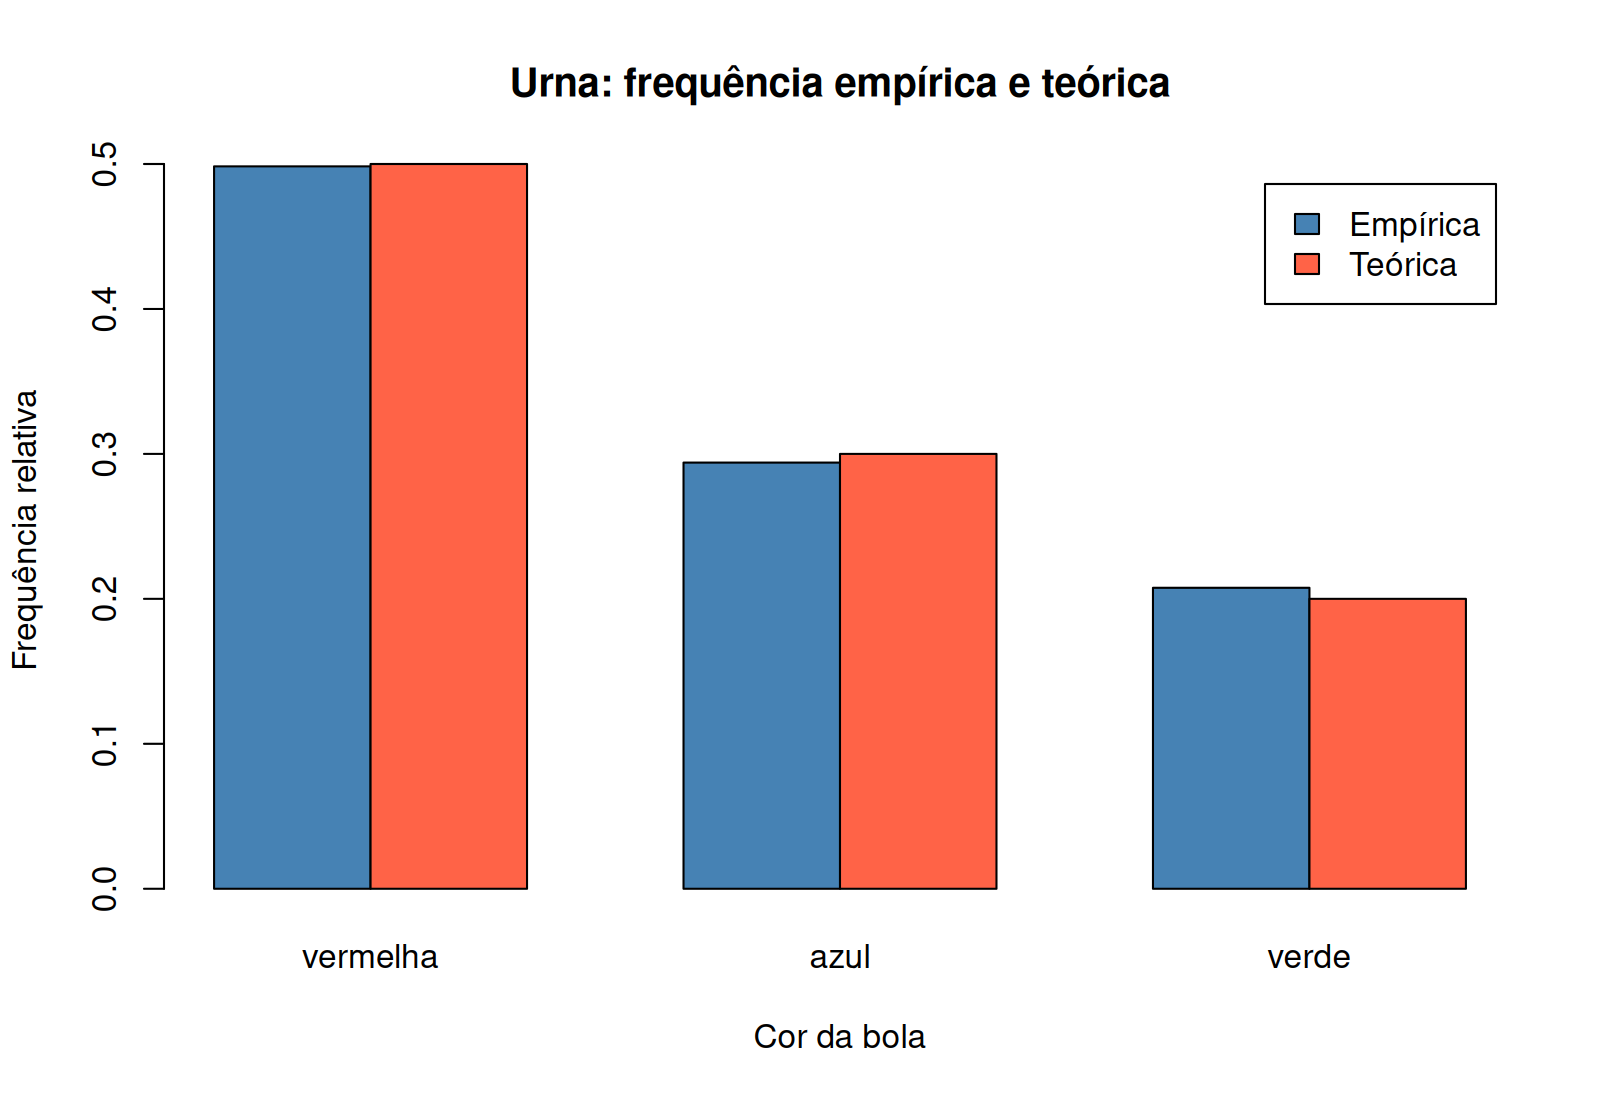
\includegraphics[width=0.8\textwidth]{secoes/02_simulacao/imagens/fig_urna_freq.png}
	\caption{Frequências empírica e teórica das cores da urna.}
	\label{fig:urna}
\end{figure}

\subsection{Soma de dois dados e a média amostral}

A função \textit{replicate()} permite repetir um experimento um número grande de
vezes. Aqui, o experimento consiste em somar dois dados honestos, repetido
$n = 20000$ vezes. A soma $S = X_1 + X_2$ pode assumir os valores inteiros de $2$
a $12$. Como os dois dados são lançados de forma independente e cada um tem seis
faces, existem $6 \times 6 = 36$ pares ordenados igualmente prováveis, e a
probabilidade de uma soma $s$ é a razão entre o número de pares que a produzem e o
total de $36$, conforme a Equação~\ref{eq:prob_soma}.

\begin{equation}
	P(S = s) = \frac{N(s)}{36}, \qquad N(s) = 6 - |s - 7|, \qquad s = 2, 3, \ldots, 12
	\label{eq:prob_soma}
\end{equation}

Na Equação~\ref{eq:prob_soma}, $N(s)$ é o número de pares $(i, j)$ com
$i + j = s$. Esse número cresce de $1$, para a soma $2$, até o máximo de $6$, para
a soma $7$, e decresce de forma simétrica até $1$, para a soma $12$, o que dá à
distribuição o formato triangular e torna a soma $7$ a mais provável
\cite{ross2010probabilidade}. O Listing~\ref{lst:soma} repete o experimento com
\textit{replicate()}.

\begin{lstlisting}[caption={Distribuição da soma de dois dados com \textit{replicate()}.}, label={lst:soma}]
n_rep <- 20000
soma <- replicate(n_rep, sum(sample(1:6, size = 2, replace = TRUE)))

freq_emp_soma <- table(factor(soma, levels = 2:12)) / n_rep
freq_teo_soma <- c(1, 2, 3, 4, 5, 6, 5, 4, 3, 2, 1) / 36
\end{lstlisting}

A distribuição obtida aparece na Figura~\ref{fig:soma}, que reproduz o formato
triangular esperado, com a soma $7$ sendo a mais frequente.

\begin{figure}[H]
	\centering
	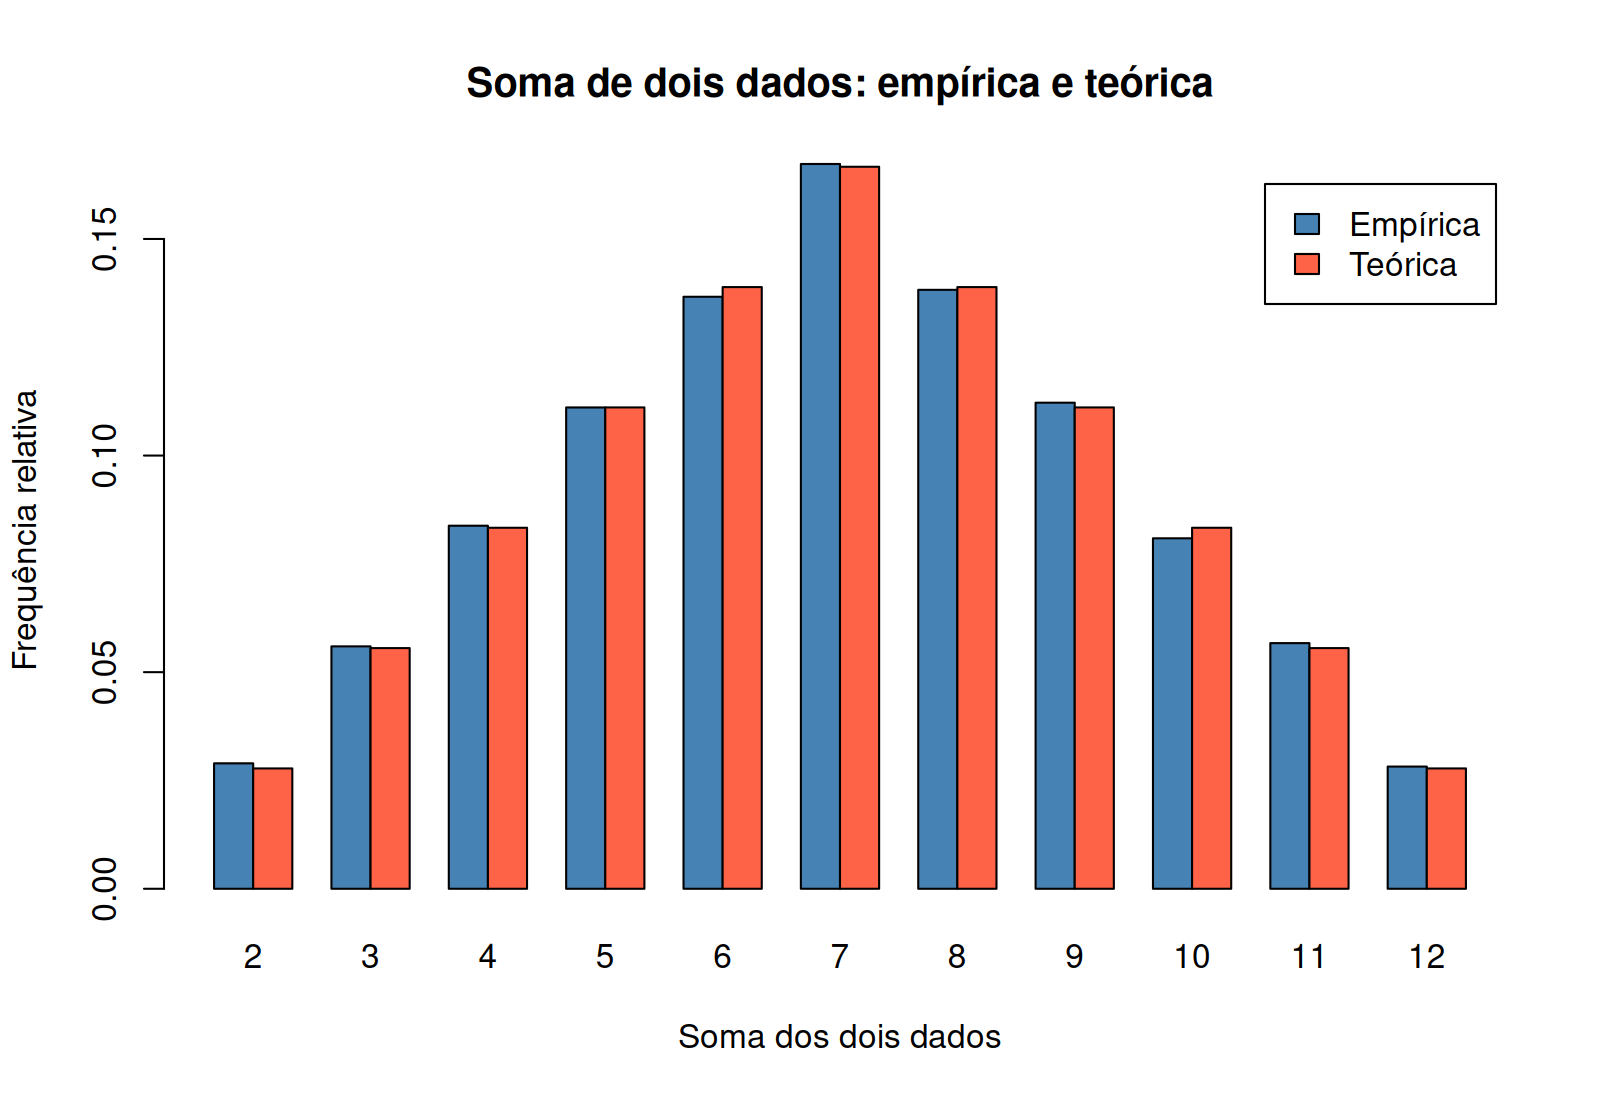
\includegraphics[width=0.8\textwidth]{secoes/02_simulacao/imagens/fig_soma_dois_dados.png}
	\caption{Distribuição empírica e teórica da soma de dois dados.}
	\label{fig:soma}
\end{figure}

A mesma simulação ilustra a convergência da média amostral, da qual a frequência
relativa da moeda é um caso particular. O valor esperado da soma é a soma dos
valores esperados de cada dado, conforme a Equação~\ref{eq:esperanca_soma}.

\begin{equation}
	E[S] = E[X_1] + E[X_2] = 3{,}5 + 3{,}5 = 7
	\label{eq:esperanca_soma}
\end{equation}

Pela Lei dos Grandes Números, a média acumulada das somas converge para
$E[S] = 7$ à medida que o número de repetições aumenta
\cite{ross2010probabilidade}. O Listing~\ref{lst:soma_media} acompanha essa média
acumulada.

\begin{lstlisting}[caption={Média amostral acumulada da soma de dois dados.}, label={lst:soma_media}]
media_soma <- cumsum(soma) / seq_len(n_rep)
\end{lstlisting}

A convergência é exibida na Figura~\ref{fig:soma_media}. A média amostral final
observada foi $6{,}9944$, próxima de $7$. A média acumulada oscila de forma
acentuada nas primeiras repetições e passa a se estabilizar em torno do valor
esperado, com flutuações que diminuem à medida que a amostra cresce.

\begin{figure}[H]
	\centering
	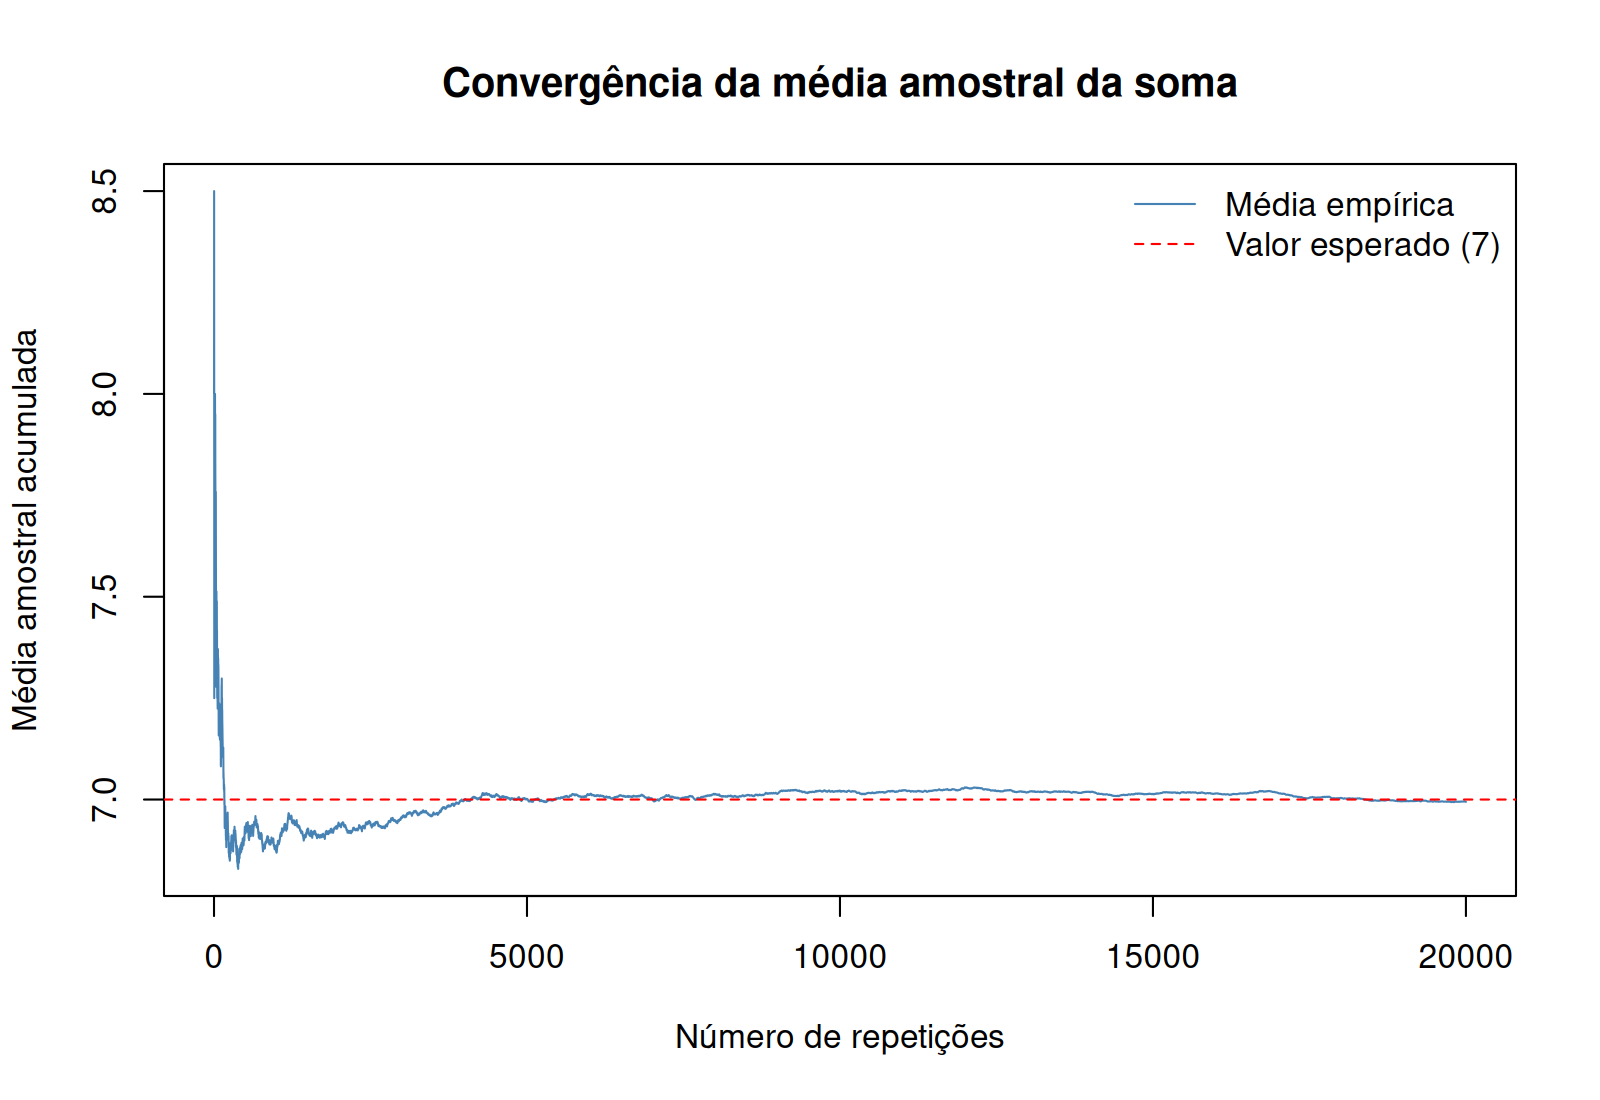
\includegraphics[width=0.8\textwidth]{secoes/02_simulacao/imagens/fig_soma_media.png}
	\caption{Convergência da média amostral da soma para $7$.}
	\label{fig:soma_media}
\end{figure}

	
	\section{Distribuições Discretas}

As distribuições discretas descrevem variáveis aleatórias que assumem valores em um
conjunto enumerável, situação comum em Computação quando o interesse recai sobre
contagens, como o número de falhas em um conjunto de requisições. Nesta seção são
apresentados os três modelos discretos mais usados, Bernoulli, binomial e Poisson,
e suas previsões teóricas são comparadas com estimativas obtidas por simulação em R.

\subsection{Conceitos fundamentais}

Uma variável aleatória $X$ é uma função $X \colon \Omega \to \mathbb{R}$ que associa
a cada resultado $\xi \in \Omega$ um número real $X(\xi)$ \cite{chan2021probability}.
Uma variável aleatória discreta assume um conjunto enumerável, finito ou infinito,
de valores, enquanto uma variável aleatória contínua assume valores em um conjunto
não enumerável \cite{harcholbalter2024probability}.

A função massa de probabilidade de uma variável aleatória discreta $X$ é definida na
Equação~\ref{eq:fmp} e atribui a cada valor possível a probabilidade de ele ser
observado. O conjunto de todos os valores possíveis de $X$ é denotado por
$X(\Omega)$.

\begin{equation}
	p_X(x) = P(X = x)
	\label{eq:fmp}
\end{equation}

\subsection{Principais distribuições discretas}

\subsubsection{Distribuição de Bernoulli}

A distribuição de Bernoulli modela um único experimento com dois resultados
possíveis, sucesso, codificado como $1$, e falha, codificado como $0$. Sua função
massa de probabilidade aparece na Equação~\ref{eq:bernoulli}, em que $0 < p < 1$ é a
probabilidade de sucesso. A esperança é $E[X] = p$ e a variância é
$\Var(X) = p(1-p)$, de modo que a variância é máxima quando $p = 0{,}5$ e se anula
nos extremos \cite{sahu2024probability}.

\begin{equation}
	p_X(0) = 1 - p, \qquad p_X(1) = p
	\label{eq:bernoulli}
\end{equation}

\subsubsection{Distribuição binomial}

A distribuição binomial descreve o número de sucessos em $n$ ensaios de Bernoulli
independentes, todos com a mesma probabilidade de sucesso $p$. Sua função massa de
probabilidade aparece na Equação~\ref{eq:binomial}, em que $\binom{n}{k}$ conta as
maneiras de escolher quais ensaios resultam em sucesso \cite{chan2021probability}. A
esperança é $E[X] = np$ e a variância é $\Var(X) = np(1-p)$.

\begin{equation}
	p_X(k) = \binom{n}{k} p^k (1 - p)^{n-k}, \qquad k = 0, 1, \ldots, n
	\label{eq:binomial}
\end{equation}

\subsubsection{Distribuição de Poisson}

A distribuição de Poisson modela o número de ocorrências de um evento em um
intervalo fixo de tempo ou espaço, quando essas ocorrências são raras e
independentes. Sua função massa de probabilidade aparece na
Equação~\ref{eq:poisson}, em que $\lambda > 0$ é a taxa média de ocorrências
\cite{chan2021probability}. Uma característica marcante é que a esperança e a
variância coincidem, $E[X] = \Var(X) = \lambda$.

\begin{equation}
	p_X(k) = \frac{\lambda^k}{k!}\, e^{-\lambda}, \qquad k = 0, 1, 2, \ldots
	\label{eq:poisson}
\end{equation}

\subsection{Modelagem de um cenário de falhas}

Para ilustrar os três modelos foi considerado um servidor cujas requisições falham
de forma independente com probabilidade $p = 0{,}05$. Cada requisição corresponde a
uma variável de Bernoulli que vale $1$ em caso de falha. O número de falhas em um
bloco de $n = 20$ requisições segue uma distribuição binomial de parâmetros $n$ e
$p$, com esperança $np = 1$. O número de falhas observadas em um intervalo de um
minuto, supondo uma taxa média de $\lambda = 2$ falhas por minuto, é modelado por
uma distribuição de Poisson.

\subsection{Simulação e resultados}

As distribuições foram simuladas com $20000$ repetições e as frequências empíricas
foram comparadas com as probabilidades teóricas. O Listing~\ref{lst:disc_gera} gera
as amostras da binomial e da Poisson.

\begin{lstlisting}[caption={Simulação das distribuições binomial e de Poisson.}, label={lst:disc_gera}]
p <- 0.05
n_req <- 20
lambda <- 2
n_rep <- 20000

falhas_binom <- rbinom(n_rep, size = n_req, prob = p)
falhas_pois  <- rpois(n_rep, lambda)
\end{lstlisting}

A Figura~\ref{fig:disc_binomial} e a Figura~\ref{fig:disc_poisson} comparam as
frequências empíricas com as probabilidades teóricas da binomial e da Poisson. Em
ambos os casos as barras empíricas praticamente coincidem com as teóricas, o que
confirma que a simulação reproduz os modelos.

\begin{figure}[H]
	\centering
	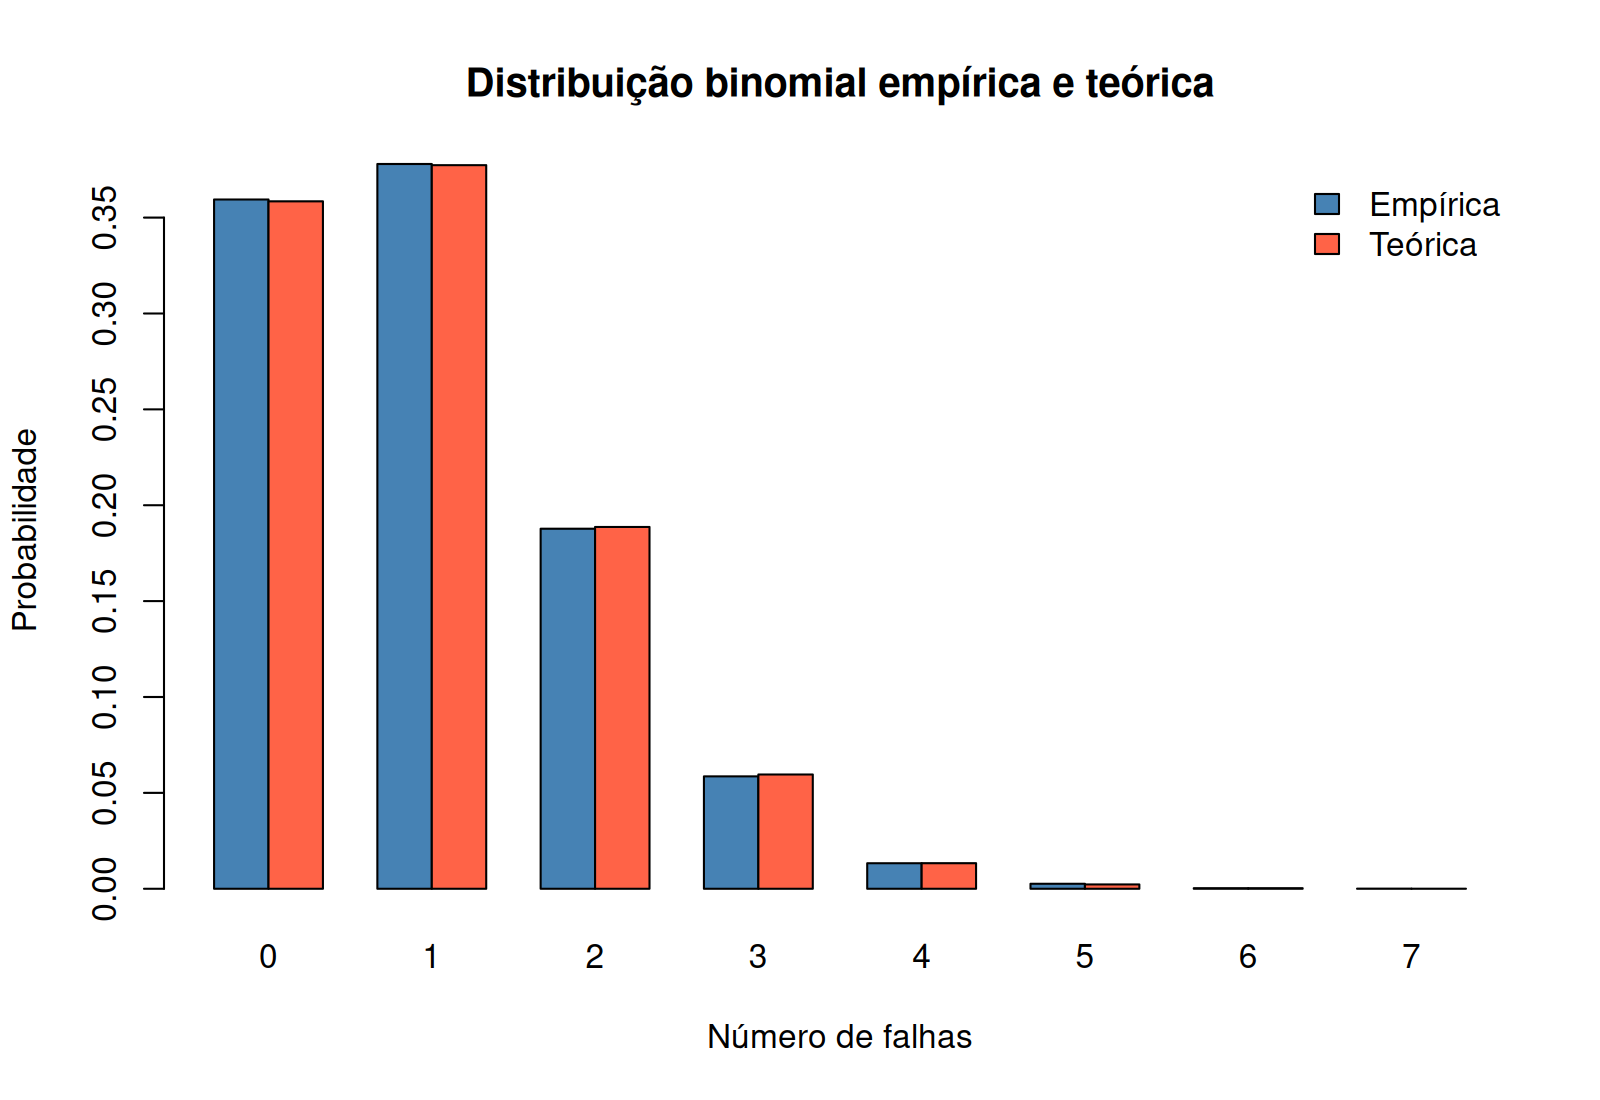
\includegraphics[width=0.8\textwidth]{secoes/03_distribuicoes_discretas/imagens/fig_binomial.png}
	\caption{Distribuição binomial empírica e teórica para $n = 20$ e $p = 0{,}05$.}
	\label{fig:disc_binomial}
\end{figure}

\begin{figure}[H]
	\centering
	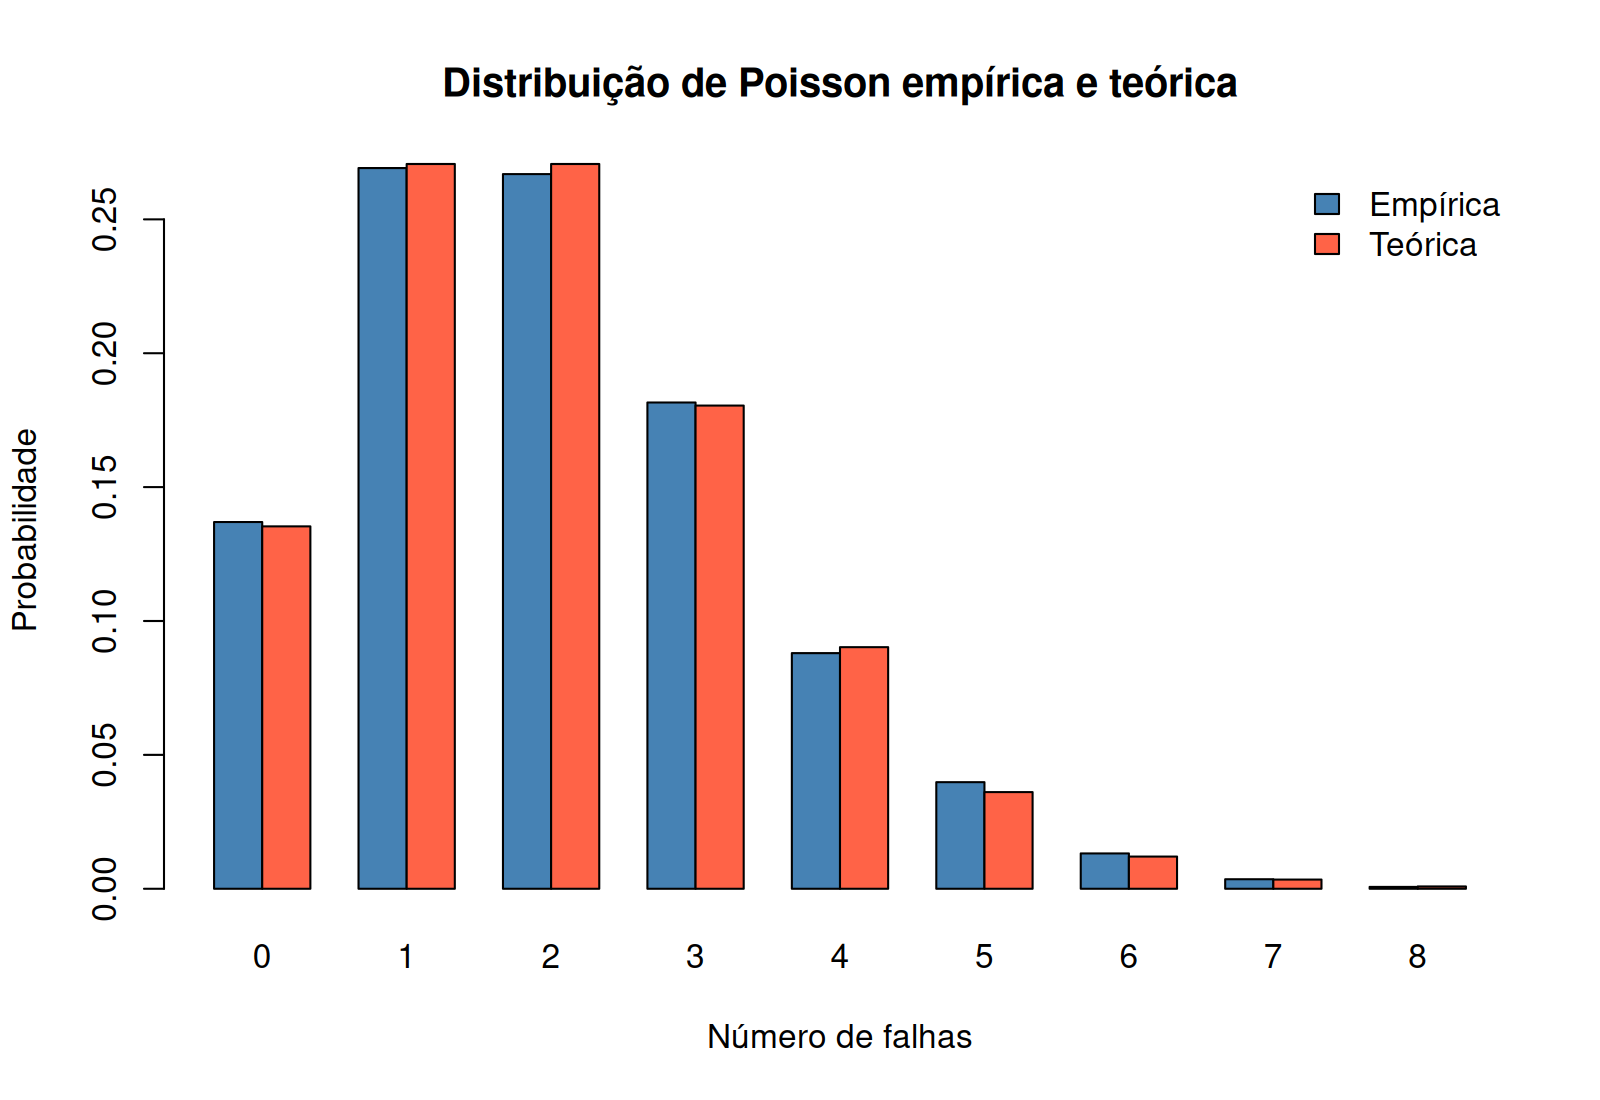
\includegraphics[width=0.8\textwidth]{secoes/03_distribuicoes_discretas/imagens/fig_poisson.png}
	\caption{Distribuição de Poisson empírica e teórica para $\lambda = 2$.}
	\label{fig:disc_poisson}
\end{figure}

A Tabela~\ref{tab:disc_medias} compara a média amostral de cada distribuição com a
esperança teórica. As diferenças aparecem apenas a partir da segunda casa decimal,
coerente com a Lei dos Grandes Números \cite{ross2010probabilidade}.

\begin{table}[H]
	\centering
	\caption{Média amostral e esperança teórica das distribuições simuladas.}
	\begin{tabular}{lcc}
		\toprule
		& Binomial $(20;\,0{,}05)$ & Poisson $(2)$ \\
		\midrule
		Empírica & 0,9976 & 2,0098 \\
		Teórica  & 1,0000 & 2,0000 \\
		\bottomrule
	\end{tabular}
	\label{tab:disc_medias}
\end{table}

A Figura~\ref{fig:disc_media} acompanha a média amostral acumulada do número de
falhas da binomial ao longo das repetições. A curva oscila bastante no início e se
estabiliza em torno do valor teórico $np = 1$ conforme o número de repetições
aumenta, o que ilustra a convergência prevista pela Lei dos Grandes Números.

\begin{figure}[H]
	\centering
	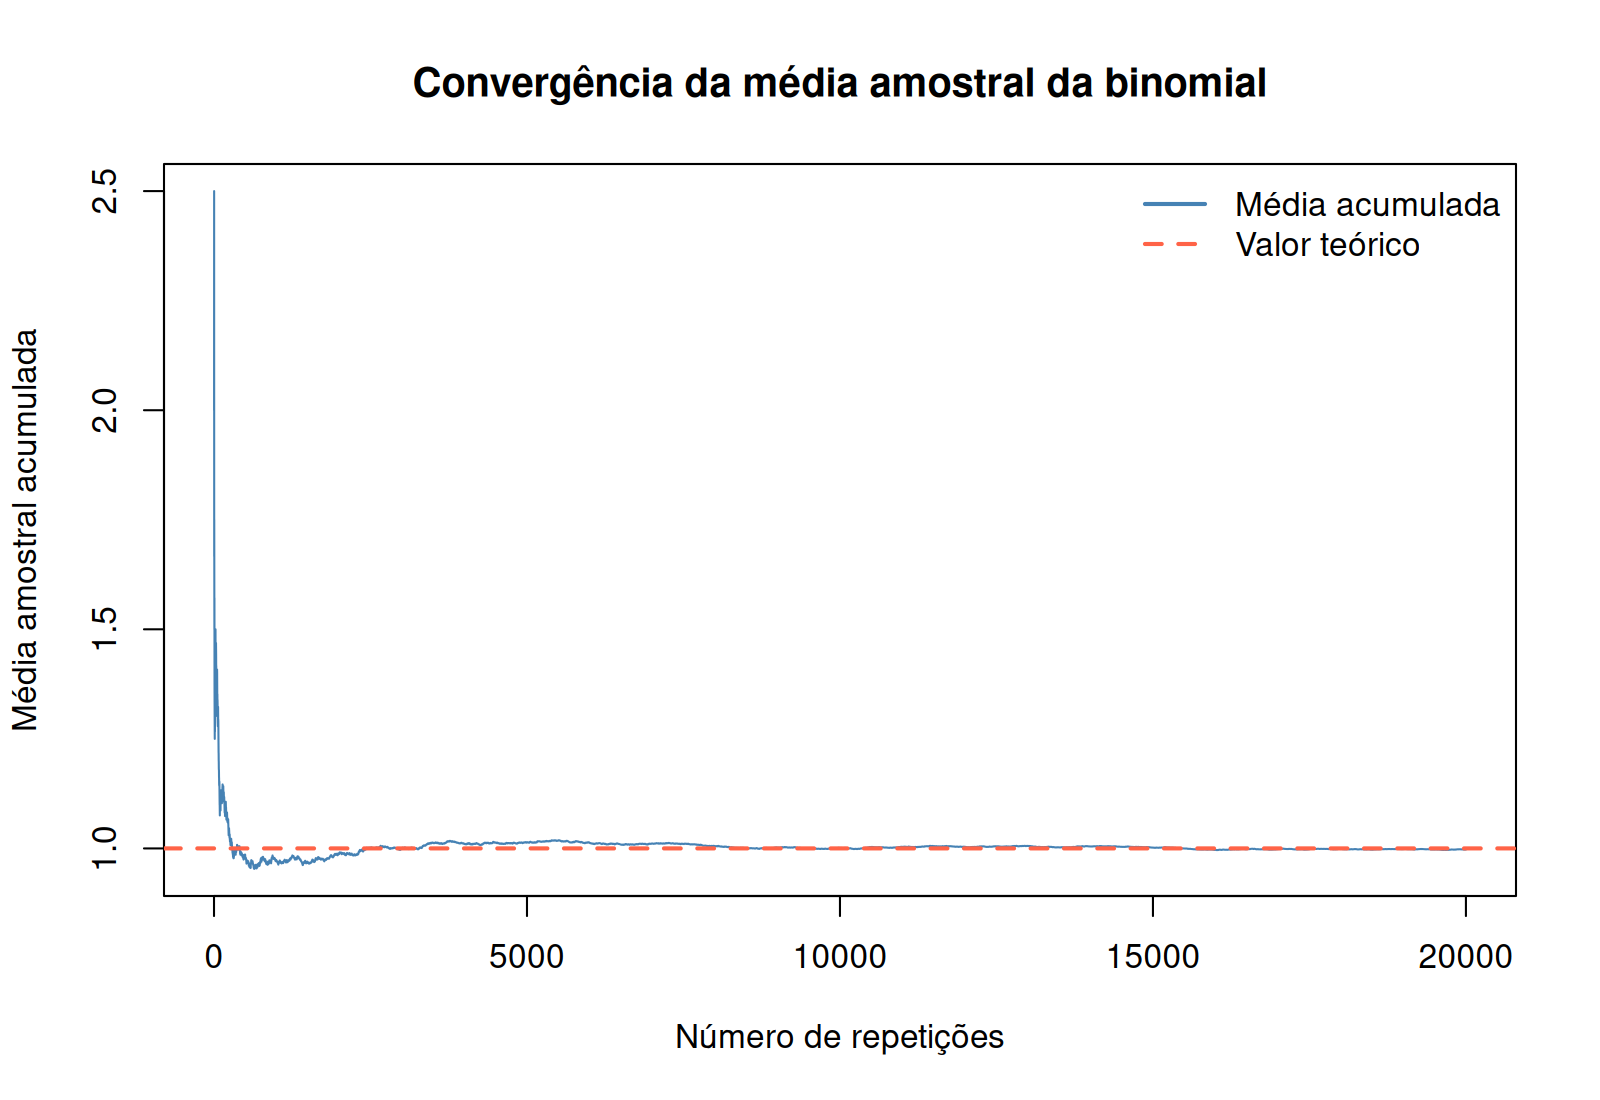
\includegraphics[width=0.8\textwidth]{secoes/03_distribuicoes_discretas/imagens/fig_media_discreta.png}
	\caption{Convergência da média amostral da binomial para a esperança $np = 1$.}
	\label{fig:disc_media}
\end{figure}

	
	\section{Distribuições Contínuas: Normal, Uniforme e Exponencial}


	\section{Calculo de Esperança, Variância e Lei dos Grandes Números}
Esta seção aborda a validação empírica dos conceitos de Esperança Matemática ($E[X]$) e Variância ($\Var(X)$), estendendo a análise para a verificação do fenômeno da estabilidade estatística ditado pela Lei dos Grandes Números (LGN).

\subsection{Definições Teóricas}

A Lei dos Grandes Números garante que a média amostral de ensaios independentes converge para a média teórica populacional quando o número de ensaios tende ao infinito:
\begin{equation}
    P\left( \lim_{k \to \infty} \bar{X}_k = \mu \right) = 1
\end{equation}

Utilizou-se uma variável aleatória contínua $X \sim Exp(\lambda = 0.2)$. Os parâmetros teóricos de controle de longa duração são definidos matematicamente por:
\begin{align}
    E[X] &= \frac{1}{\lambda} = \frac{1}{0.2} = 5.0000 \\
    \Var(X) &= \frac{1}{\lambda^2} = \frac{1}{0.04} = 25.0000
\end{align}

\subsection{Resultados e Análise Crítica}

Após a execução da simulação computacional para $K = 10.000$ ensaios independentes, os valores empíricos organizados comparativamente são apresentados na Tabela \ref{tab:t4_comparativo}.

\begin{table}[H]
    \centering
    \caption{Comparação entre Parâmetros Teóricos e Estimativas Empíricas ($K=10.000$).}
    \label{tab:t4_comparativo}
    \vspace{2mm}
    \begin{tabular}{lccc}
        \toprule
        \textbf{Métrica} & \textbf{Valor Teórico} & \textbf{Estimativa Empírica} & \textbf{Erro Relativo (\%)} \\ \midrule
        Esperança $E[X]$ & 5,0000 & 5,0189 & 0,38\% \\
        Variância $\Var(X)$ & 25,0000 & 24,9941 & 0,02\% \\ \bottomrule
    \end{tabular}
\end{table}

A visualização do processo dinâmico de convergência da média móvel ao longo das iterações é apresentada na Figura \ref{fig:t4_grafico}.

\begin{figure}[H]
    \centering
    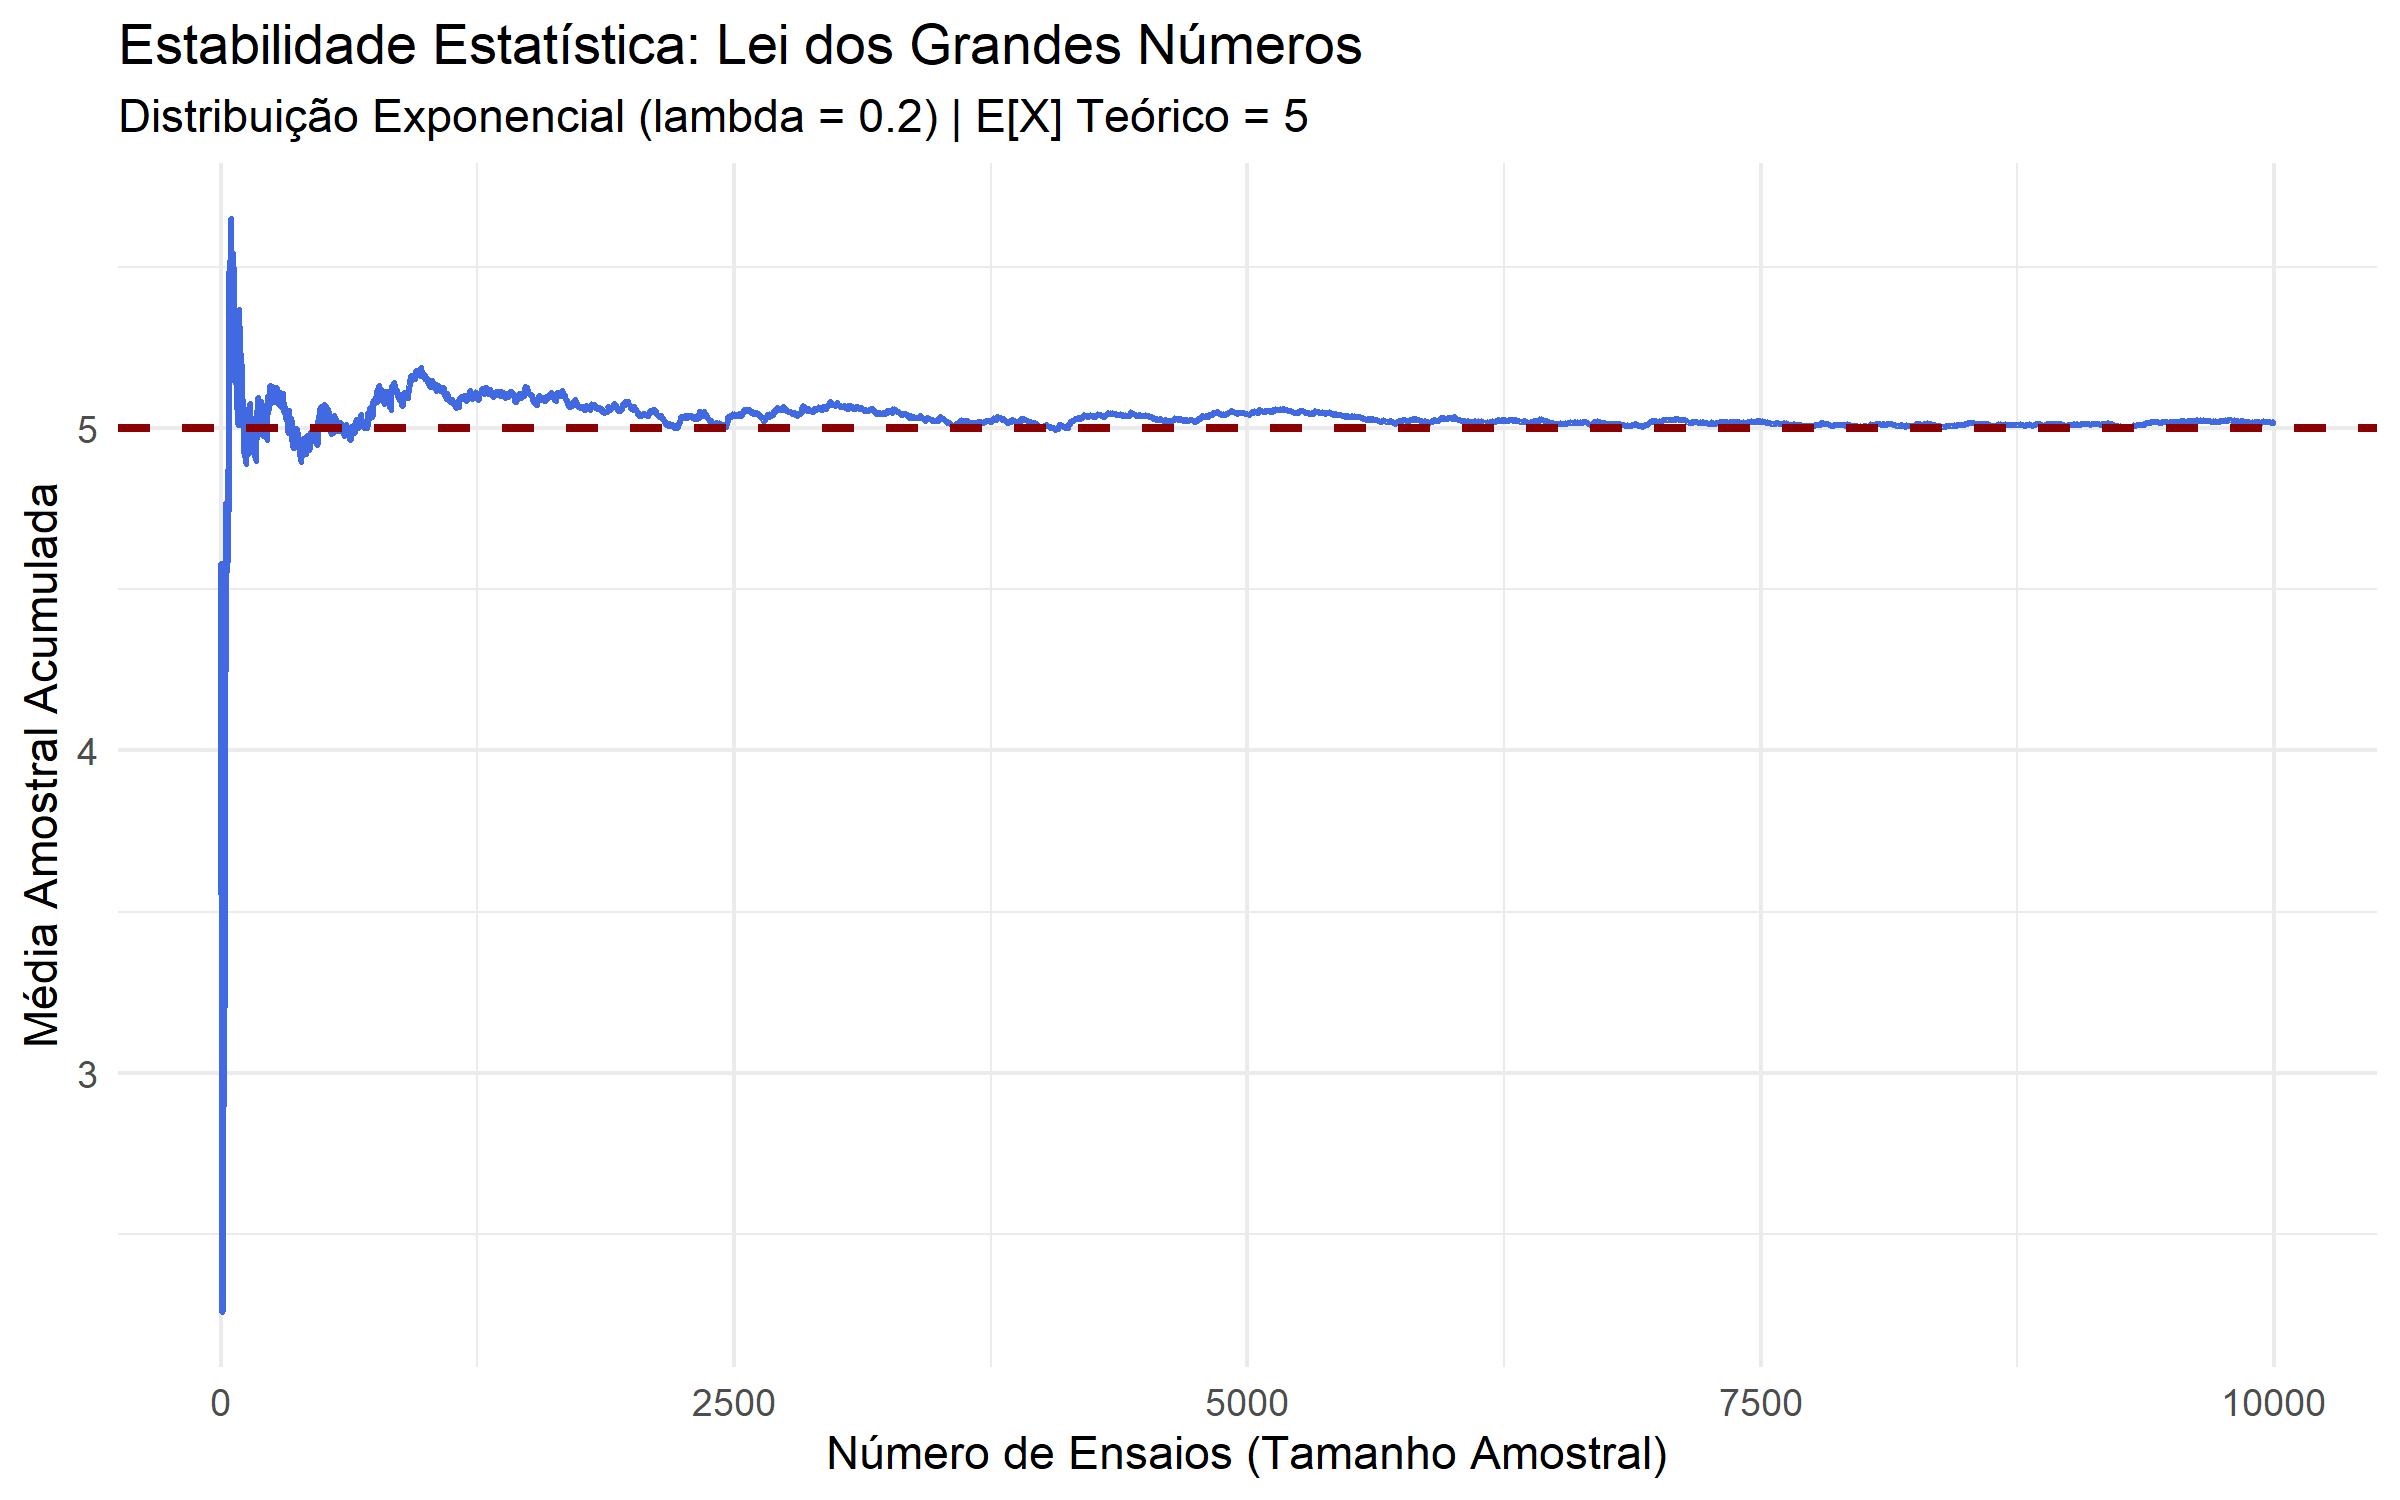
\includegraphics[width=0.85\textwidth]{imagens/t4_lei_grandes_numeros.png}
    \caption{Evolução da média amostral acumulada em função do número de ensaios, demonstrando a convergência assintótica para a expectativa teórica.}
    \label{fig:t4_grafico}
\end{figure}

A interpretação do comportamento da curva permite extrair conclusões científicas sobre a estabilidade estatística:
\begin{itemize}
    \item \textbf{Flutuações Iniciais (Baixo $K$):} Nos primeiros ensaios, a variabilidade do estimador é agressiva. Como a variância da distribuição original é alta ($\Var(X) = 25$), a ocorrência de valores extremos desloca bruscamente a linha da média móvel.
    \item \textbf{Amortecimento:} À medida que o tamanho amostral cresce, o efeito de novos sorteios individuais isolados passa a ser diluído pelo denominador crescente da média móvel.
    \item \textbf{Convergência:} Próximo a $K = 10.000$, as oscilações tornam-se imperceptíveis, tangenciando a linha teórica. O baixíssimo erro relativo obtido valida o funcionamento das simulações computacionais estocásticas.
\end{itemize}

O código-fonte utilizado para esta análise encontra-se disponível no Código \ref{lst:script_t4}.

\begin{lstlisting}[language=R, caption={Validação da Lei dos Grandes Números (T4).}, label=lst:script_t4]
# T4: Esperança, Variância e Lei dos Grandes Números
set.seed(123)

if(!require(ggplot2)) install.packages("ggplot2")
library(ggplot2)

lambda <- 0.2
K <- 10000
mu_teorica <- 1 / lambda

amostras <- rexp(K, rate = lambda)
medias_acumuladas <- cumsum(amostras) / (1:K)

df_lgn <- data.frame(Ensaio = 1:K, Media_Acumulada = medias_acumuladas)

p_lgn <- ggplot(df_lgn, aes(x = Ensaio, y = Media_Acumulada)) +
  geom_line(color = "royalblue", linewidth = 0.7) +
  geom_hline(yintercept = mu_teorica, color = "darkred", linetype = "dashed", linewidth = 1) +
  labs(title = "Estabilidade Estatística: Lei dos Grandes Números",
       x = "Número de Ensaios (Tamanho Amostral)",
       y = "Média Amostral Acumulada") +
  theme_minimal()

ggsave("imagens/t4_lei_grandes_numeros.png", p_lgn, width = 8, height = 5)
\end{lstlisting}
    

	\section{Probabilidade Condicional, Independência e Teorema de Bayes}
    

	\section{Atividade Integradora Final}

\subsection{Filtro bayesiano de spam}

\subsubsection{Descrição do problema e hipóteses probabilísticas}

A filtragem de mensagens indesejadas é um problema clássico de classificação
probabilística em Computação. Cada mensagem de correio eletrônico deve ser
atribuída a uma de duas classes, spam, a mensagem indesejada, ou não spam, a
mensagem legítima. O classificador observa apenas as palavras presentes na
mensagem e precisa decidir, sob incerteza, a qual classe ela pertence. O
classificador bayesiano ingênuo é uma das abordagens mais usadas para essa
tarefa \cite{metsis2006spam}.

O modelo parte de um vocabulário fixo de $d$ palavras escolhidas de antemão,
como \textit{grátis}, \textit{promoção} e \textit{reunião}. Cada mensagem é então
representada por um vetor binário $x = (x_1, \ldots, x_d)$, em que $x_j = 1$ indica
que a palavra de índice $j$ do vocabulário aparece na mensagem e $x_j = 0$ indica
que ela não aparece. O método assume duas hipóteses probabilísticas, a primeira é
que cada classe tem uma probabilidade a priori de ocorrência, $P(S)$ para spam e
$P(\bar{S})$ para não spam. A segunda, é a hipótese
ingênua de independência condicional, segundo a qual a presença de cada palavra
é independente das demais quando a classe é conhecida \cite{sahami1998bayesian}.
Essa suposição raramente vale no texto real, já que certas palavras tendem a
ocorrer juntas, mas simplifica a modelagem e produz classificadores eficazes na
prática \cite{metsis2006spam}.

\subsubsection{Modelagem probabilística}

A decisão tem como base o Teorema de Bayes \cite{chan2021probability}. Dada a
mensagem $x$, a probabilidade a posteriori de a mensagem ser spam é obtida pela
Equação~\ref{eq:bayes_spam}.

\begin{equation}
	P(S \mid x) = \frac{P(x \mid S)\, P(S)}{P(x \mid S)\, P(S) + P(x \mid \bar{S})\, P(\bar{S})}
	\label{eq:bayes_spam}
\end{equation}

Na Equação~\ref{eq:bayes_spam}, $P(x \mid S)$ é a verossimilhança da mensagem sob
a classe spam. Sob a hipótese de independência condicional, essa verossimilhança
é o produto das probabilidades de cada palavra, conforme a
Equação~\ref{eq:nb_verossimilhanca}, em que $\theta_{jc} = P(x_j = 1 \mid c)$ é a
probabilidade de a palavra $j$ aparecer em uma mensagem da classe $c$.

\begin{equation}
	P(x \mid c) = \prod_{j=1}^{d} \theta_{jc}^{\,x_j} \, (1 - \theta_{jc})^{\,1 - x_j},
	\qquad c \in \{S, \bar{S}\}
	\label{eq:nb_verossimilhanca}
\end{equation}

A mensagem é classificada como spam quando $P(S \mid x) > 0{,}5$. Como a
verossimilhança da Equação~\ref{eq:nb_verossimilhanca} é um produto sobre as
palavras, a probabilidade a posteriori pode ser atualizada a cada palavra
observada.

As probabilidades $\theta_{jc}$ não são conhecidas e precisam ser estimadas a
partir de um conjunto de treinamento. A estimativa adotada é a frequência
relativa da Equação~\ref{eq:theta_freq}, em que $n_{jc}$ é o número de mensagens
da classe $c$ que contêm a palavra $j$ e $n_c$ é o total de mensagens da classe
$c$. É comum corrigir essa estimativa com a suavização de Laplace, que soma
contagens fixas ao numerador e ao denominador para evitar valores iguais a zero,
os quais anulariam o produto da Equação~\ref{eq:nb_verossimilhanca}. Neste
experimento toda palavra aparece em ambas as classes, de modo que
nenhuma estimativa é zero e a frequência relativa é usada diretamente.

\begin{equation}
	\hat{\theta}_{jc} = \frac{n_{jc}}{n_c}
	\label{eq:theta_freq}
\end{equation}

\subsubsection{Implementação em R}

Para validar o método, os dados foram gerados de forma controlada. As
probabilidades verdadeiras, tanto a priori de cada classe quanto a probabilidade
de cada palavra em cada classe, foram escolhidas de antemão para representar um
cenário plausível e servem de referência conhecida. A partir delas, cada mensagem
teve sua classe sorteada pela priori e, em seguida, a presença de cada palavra foi
sorteada por uma variável de Bernoulli com a probabilidade da classe
correspondente, o que impõe por construção a independência condicional. O
classificador não usa essas probabilidades verdadeiras, estimando-as apenas a
partir das mensagens geradas, o que permite verificar ao final se as estimativas
recuperam os valores escolhidos. Foram geradas $4000$ mensagens para treino e
$2000$ para teste, com $P(S) = 0{,}4$ e um vocabulário de dez palavras. O
Listing~\ref{lst:spam_gerar} mostra a geração das mensagens e a estimação das
probabilidades.

\begin{lstlisting}[caption={Geração das mensagens e estimação das probabilidades.}, label={lst:spam_gerar}]
gerar_emails <- function(n) {
  classe <- sample(c("spam", "nao_spam"), size = n, replace = TRUE,
                   prob = c(prior_spam, prior_nao_spam))
  X <- matrix(0L, nrow = n, ncol = length(palavras))
  for (j in seq_along(palavras)) {
    p <- ifelse(classe == "spam", prob_spam[j], prob_nao_spam[j])
    X[, j] <- rbinom(n, size = 1, prob = p)
  }
  list(classe = classe, X = X)
}

estimar_prob <- function(X, classe, alvo) {
  Xc <- X[classe == alvo, , drop = FALSE]
  colSums(Xc) / nrow(Xc)
}
\end{lstlisting}

A classificação calcula a probabilidade a posteriori da
Equação~\ref{eq:bayes_spam} a partir do produto de verossimilhança da
Equação~\ref{eq:nb_verossimilhanca} ponderado pelas probabilidades a priori,
conforme o Listing~\ref{lst:spam_post}.

\begin{lstlisting}[caption={Probabilidade a posteriori e classificação.}, label={lst:spam_post}]
verossimilhanca <- function(X, prob) {
  apply(X, 1, function(x) prod(prob^x * (1 - prob)^(1 - x)))
}
posterior_spam <- function(X) {
  peso_spam     <- prior_spam_est     * verossimilhanca(X, prob_spam_est)
  peso_nao_spam <- prior_nao_spam_est * verossimilhanca(X, prob_nao_spam_est)
  peso_spam / (peso_spam + peso_nao_spam)
}
pred <- ifelse(posterior_spam(teste$X) > 0.5, "spam", "nao_spam")
\end{lstlisting}

\subsubsection{Resultados e interpretação}

As probabilidades estimadas no treino ficaram próximas das teóricas, com uma
diferença abaixo de $0{,}02$, coerente com o estimador
da Equação~\ref{eq:theta_freq}. A priori de spam foi estimada em $0{,}403$, contra o
valor teórico $0{,}4$. A Tabela~\ref{tab:spam_conf} apresenta a matriz de
confusão obtida no conjunto de teste.

\begin{table}[H]
	\centering
	\caption{Matriz de confusão do classificador no conjunto de teste.}
	\begin{tabular}{lcc}
		\toprule
		Classe real & Predito não spam & Predito spam \\
		\midrule
		Não spam & 1108 & 58 \\
		Spam     & 73   & 761 \\
		\bottomrule
	\end{tabular}
	\label{tab:spam_conf}
\end{table}

A acurácia global foi de $0{,}9345$. A taxa de falsos positivos, mensagens
legítimas classificadas como spam, foi de $0{,}0497$, e a taxa de falsos
negativos, spam que passou pelo filtro, foi de $0{,}0875$. A
Figura~\ref{fig:spam_posterior} mostra a distribuição da probabilidade a
posteriori nas duas classes reais. As mensagens não spam ficam concentradas
próximo de zero e as de spam próximo de um, com poucas mensagens na região
ambígua em torno do limiar, o que sustenta a separação entre as classes.

\begin{figure}[H]
	\centering
	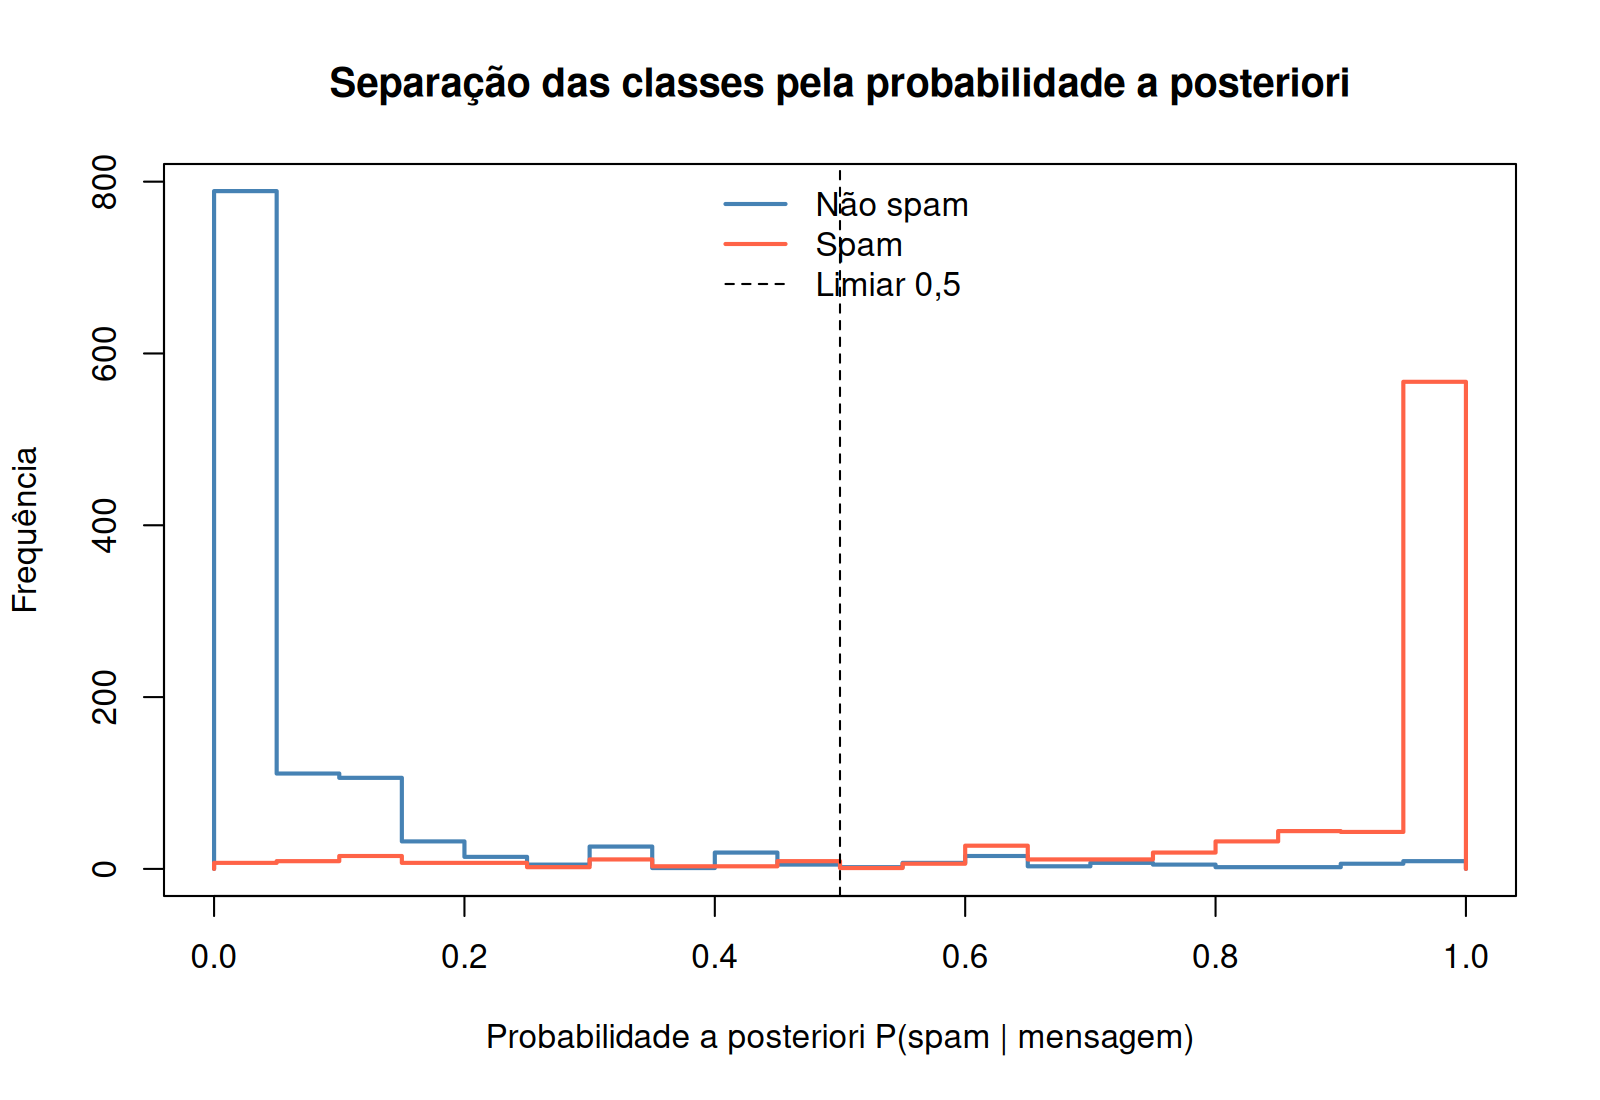
\includegraphics[width=0.8\textwidth]{secoes/07_atividade_integradora/atv_1/imagens/fig_spam_posterior.png}
	\caption{Distribuição da probabilidade a posteriori por classe real.}
	\label{fig:spam_posterior}
\end{figure}

A escolha do limiar envolve um equilíbrio entre os dois tipos de erro. Em um
filtro de spam, o falso positivo costuma ser mais grave que o falso negativo,
pois descarta uma mensagem legítima \cite{sahami1998bayesian}. A
Figura~\ref{fig:spam_limiar} mostra que
elevar o limiar reduz os falsos positivos ao custo de aumentar os falsos
negativos, permitindo ajustar o filtro à tolerância desejada.

\begin{figure}[H]
	\centering
	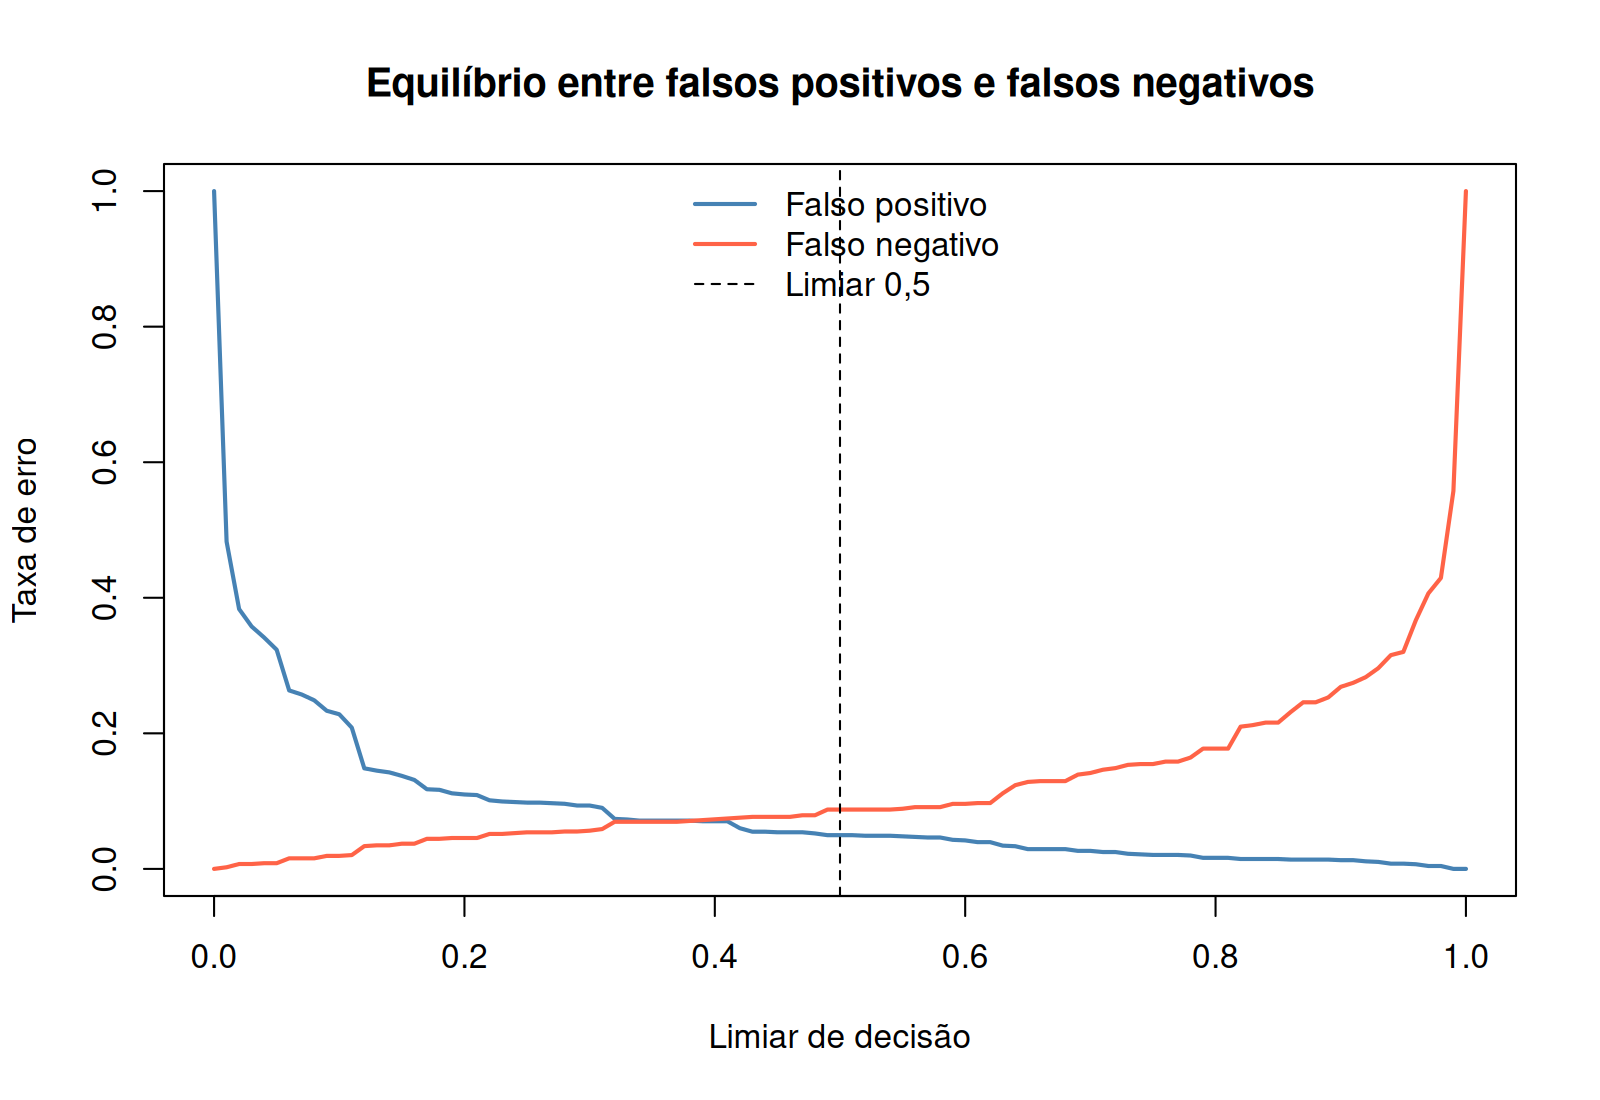
\includegraphics[width=0.8\textwidth]{secoes/07_atividade_integradora/atv_1/imagens/fig_spam_limiar.png}
	\caption{Taxas de falso positivo e falso negativo em função do limiar.}
	\label{fig:spam_limiar}
\end{figure}

A Figura~\ref{fig:spam_sequencial} mostra como a probabilidade de spam é
atualizada palavra a palavra em uma mensagem do conjunto de teste. Ela parte da
priori $0{,}403$, e a presença de palavras típicas de spam eleva a posteriori,
enquanto a ausência de palavras típicas de
não spam também contribui como evidência, de modo que a estimativa final atinge
$0{,}997$.

\begin{figure}[H]
	\centering
	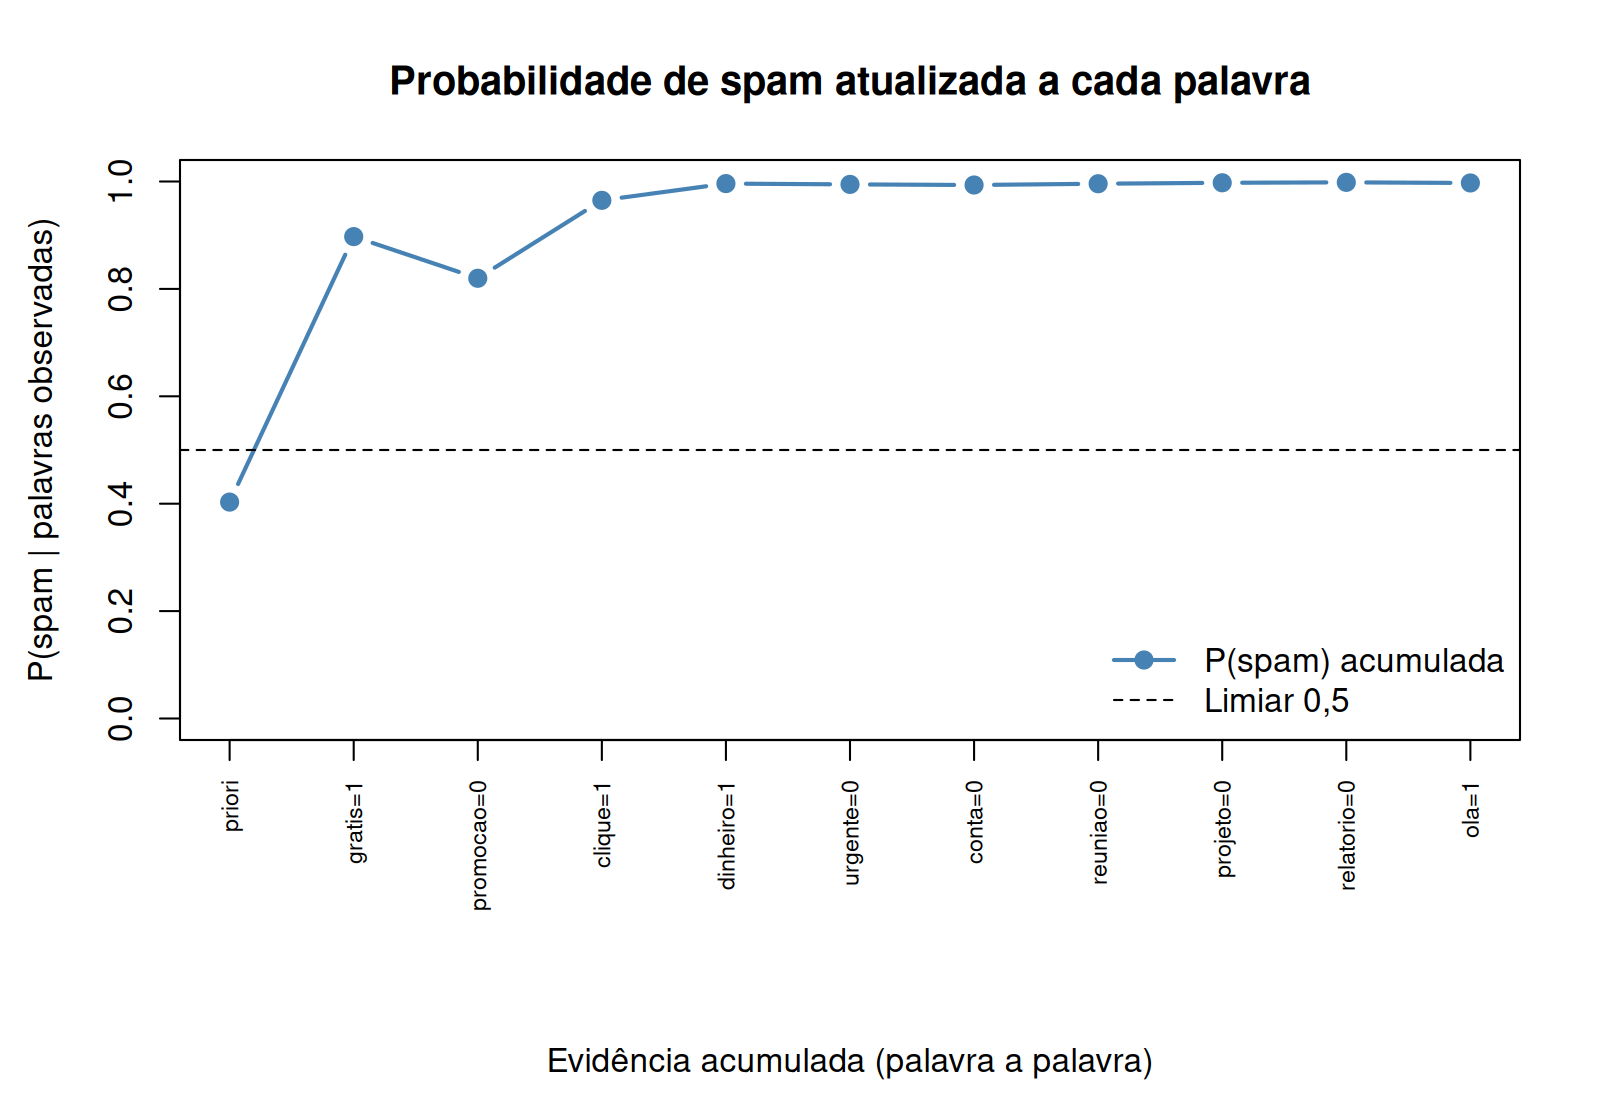
\includegraphics[width=0.8\textwidth]{secoes/07_atividade_integradora/atv_1/imagens/fig_spam_sequencial.png}
	\caption{Atualização da probabilidade a posteriori de spam, palavra a palavra.}
	\label{fig:spam_sequencial}
\end{figure}

A independência condicional vale por construção neste experimento, situação em
que as suposições do modelo são exatamente satisfeitas, o que explica a
proximidade entre as probabilidades estimadas e as teóricas e a alta acurácia. Em
mensagens reais essa hipótese geralmente é violada, pois as palavras apresentam
dependências. Ainda assim, o classificador
ingênuo mantém bom desempenho prático \cite{metsis2006spam}.


\subsection{Confiabilidade e detecção de falhas}

\subsubsection{Descrição do problema e hipóteses probabilísticas}

A confiabilidade é uma preocupação central no projeto de sistemas
computacionais, pois servidores, por exemplo, podem falhar de maneira imprevisível
e a indisponibilidade tem custo elevado. O objetivo deste estudo é quantificar a
probabilidade de um sistema permanecer em funcionamento ao longo do tempo e
avaliar o ganho obtido com a redundância de componentes.

O tempo até a falha de um componente é modelado por uma variável aleatória
contínua $T$. A hipótese probabilística central é que esse tempo segue uma
distribuição exponencial de taxa $\lambda$, o que equivale a supor uma taxa de
falha constante ao longo da vida útil \cite{harcholbalter2024probability}. Essa
escolha decorre da propriedade de falta de memória apresentada na
Equação~\ref{eq:conf_memoryless}, segundo a qual
um componente que já operou por um tempo $s$ tem a mesma distribuição de vida
restante de um componente novo. A segunda hipótese é que as falhas dos diversos
componentes são independentes entre si, o que permite combinar as probabilidades
individuais por produto.

\begin{equation}
	P(T > s + t \mid T > s) = P(T > t), \qquad s, t \ge 0
	\label{eq:conf_memoryless}
\end{equation}

\subsubsection{Modelagem probabilística}

A confiabilidade de um componente é a probabilidade de ele ainda estar em
funcionamento no instante $t$, dada na Equação~\ref{eq:conf_exp}. O tempo médio
até a falha é a esperança da distribuição exponencial e vale
$1/\lambda$.

\begin{equation}
	R(t) = P(T > t) = e^{-\lambda t}, \qquad E[T] = \frac{1}{\lambda}
	\label{eq:conf_exp}
\end{equation}

Sistemas reais combinam vários componentes. Em um arranjo em série todos os
componentes precisam funcionar, de modo que o sistema falha assim que o primeiro
componente falha. Sob independência, a confiabilidade do arranjo em série é o
produto das confiabilidades, conforme a Equação~\ref{eq:conf_serie}
\cite{ross2010probabilidade}.

\begin{equation}
	R_{\text{serie}}(t) = \prod_{i=1}^{n} R_i(t)
	\label{eq:conf_serie}
\end{equation}

Em um arranjo em paralelo, ou redundante, o sistema funciona enquanto ao menos um
componente estiver operante, falhando apenas quando o último falha. A
confiabilidade é o complemento do produto das probabilidades de falha de cada
componente, conforme a Equação~\ref{eq:conf_paralelo} \cite{ross2010probabilidade}.

\begin{equation}
	R_{\text{paralelo}}(t) = 1 - \prod_{i=1}^{n} \bigl(1 - R_i(t)\bigr)
	\label{eq:conf_paralelo}
\end{equation}

\subsubsection{Implementação em R}

A confiabilidade foi estimada por simulação de Monte Carlo. Foram gerados os
tempos de vida de $100000$ sistemas, cada um com seus componentes exponenciais
independentes de taxa $\lambda = 0{,}1$, o que corresponde a um tempo médio até a
falha de $10$ por componente. O tempo até a falha de cada arranjo decorre diretamente da sua
estrutura, sendo o mínimo dos tempos no caso em série e o máximo no caso em
paralelo. O Listing~\ref{lst:conf_gera} gera os tempos de vida e os arranjos.

\begin{lstlisting}[caption={Geração dos tempos de vida e dos arranjos.}, label={lst:conf_gera}]
lambda <- 0.1
N      <- 100000
comp   <- matrix(rexp(N * 3, rate = lambda), nrow = N, ncol = 3)

vida_unico <- comp[, 1]
vida_serie <- pmin(comp[, 1], comp[, 2], comp[, 3])
vida_paral <- pmax(comp[, 1], comp[, 2], comp[, 3])
\end{lstlisting}

A confiabilidade empírica em um instante $t$ é a fração de sistemas que ainda não
falharam, conforme o Listing~\ref{lst:conf_emp}.

\begin{lstlisting}[caption={Confiabilidade empírica em função do tempo.}, label={lst:conf_emp}]
t_grid <- seq(0, 40, by = 0.5)
R_emp  <- function(vida) sapply(t_grid, function(t) mean(vida > t))
\end{lstlisting}

\subsubsection{Resultados e interpretação}

A Tabela~\ref{tab:conf_mtbf} compara o tempo médio até a falha de cada arranjo. O
arranjo em série reduz esse tempo de $10$ para cerca de $3{,}3$, pois basta uma falha
para derrubar o sistema, enquanto o arranjo em paralelo o eleva para cerca de
$18{,}3$. Em todos os arranjos a estimativa empírica difere do valor teórico
apenas na segunda casa decimal.

\begin{table}[H]
	\centering
	\caption{Tempo médio até a falha por arranjo, com $\lambda = 0{,}1$.}
	\begin{tabular}{lccc}
		\toprule
		& Único & Série de 3 & Paralelo de 3 \\
		\midrule
		Empírico & 9,9818 & 3,3173 & 18,3247 \\
		Teórico  & 10,0000 & 3,3333 & 18,3333 \\
		\bottomrule
	\end{tabular}
	\label{tab:conf_mtbf}
\end{table}

A Figura~\ref{fig:conf_curvas} mostra as curvas de confiabilidade dos arranjos
único, em série e em paralelo ao longo do tempo. Os pontos empíricos acompanham
as curvas teóricas, e a ordenação é clara, pois o arranjo em paralelo preserva
confiabilidade alta por muito mais tempo que o componente isolado, enquanto o
arranjo em série decai mais rápido.

\begin{figure}[H]
	\centering
	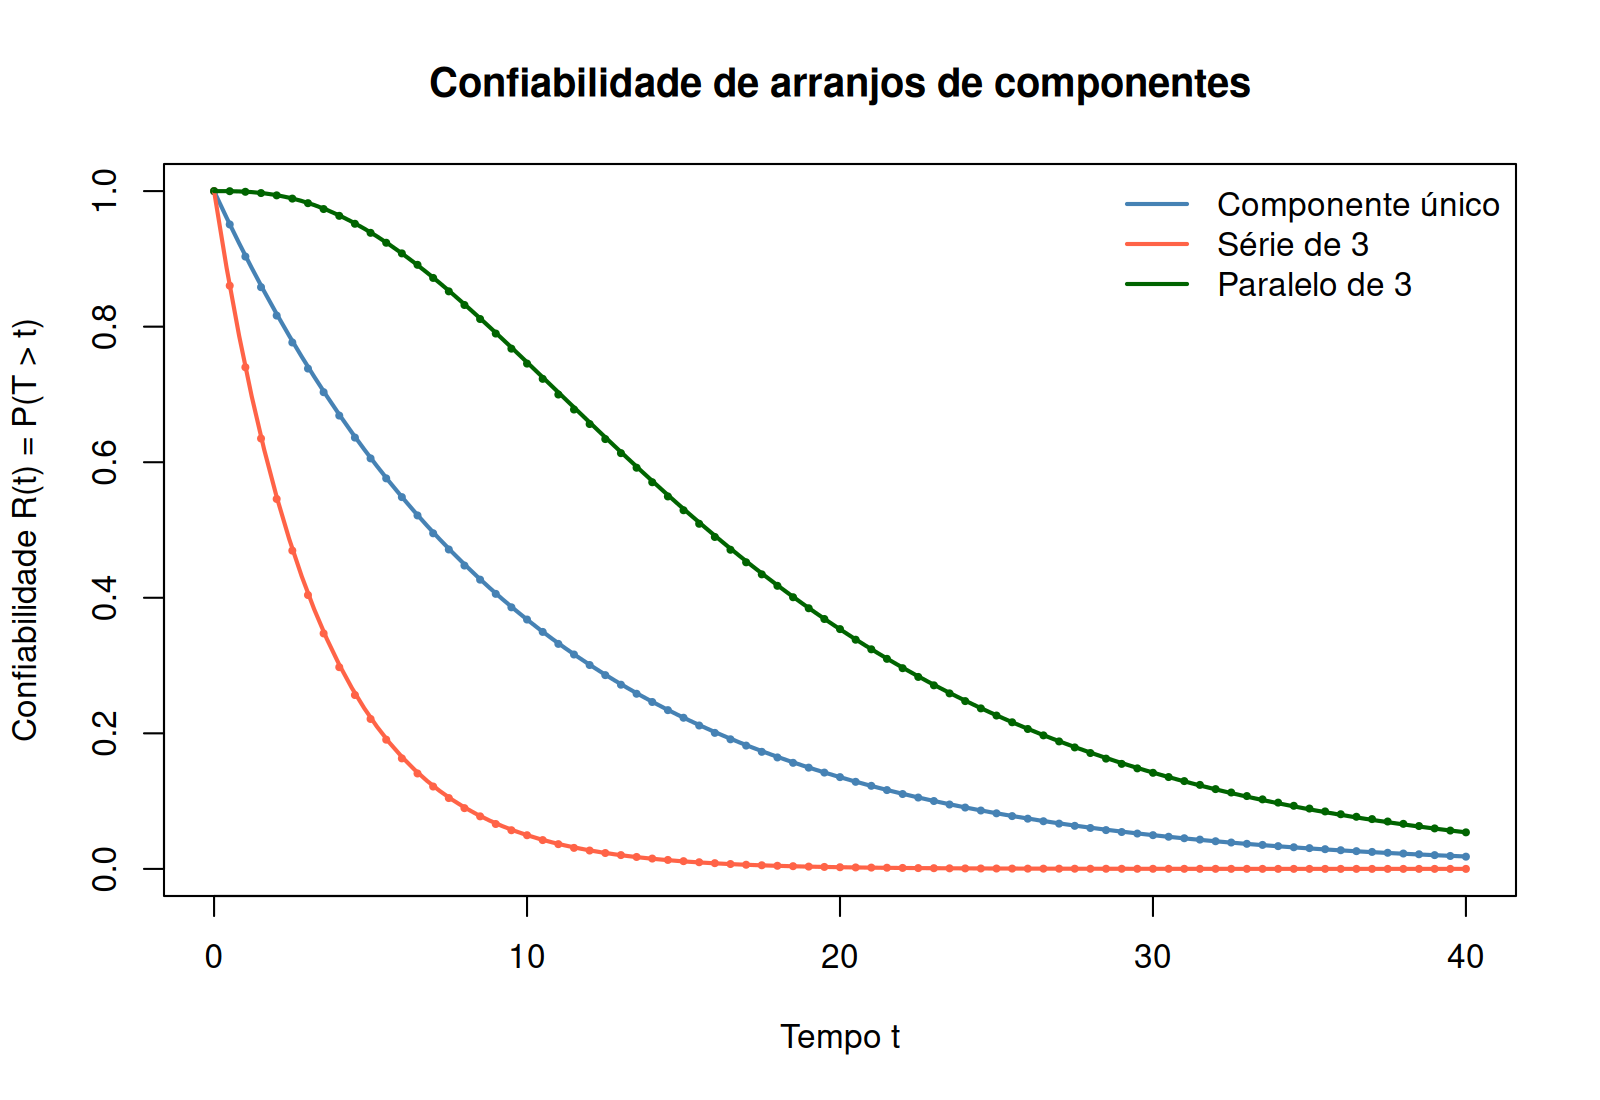
\includegraphics[width=0.8\textwidth]{secoes/07_atividade_integradora/atv_2/imagens/fig_conf_curvas.png}
	\caption{Confiabilidade $R(t)$ dos arranjos único, série e paralelo.}
	\label{fig:conf_curvas}
\end{figure}

Os valores empíricos e teóricos concordam em todos os arranjos analisados. A
comparação evidencia a relação entre custo e confiabilidade, pois a
redundância em paralelo eleva o tempo médio até a falha ao preço de mais
componentes, enquanto o arranjo em série, embora mais simples, é menos confiável
que um único componente. A hipótese de taxa de falha constante é uma
simplificação, pois na prática a chance de falha pode mudar com o tempo de uso do
componente.


	

	\section{Conclusão}

Este relatório percorreu conceitos centrais da teoria da probabilidade combinando o
tratamento teórico com experimentos computacionais em R. Em todos os estudos as
estimativas empíricas se aproximaram dos valores previstos pela teoria, e esse
acordo entre o que foi calculado e o que foi observado ilustra como a simulação pode
validar resultados analíticos.

A simulação de experimentos aleatórios mostrou que a frequência relativa de um
evento se estabiliza em torno de sua probabilidade teórica à medida que o número de
repetições cresce. O lançamento da moeda, a retirada de bolas da urna e a soma de
dois dados reproduziram as probabilidades teóricas, e a média amostral da soma
convergiu para o seu valor esperado, como prevê a Lei dos Grandes Números
\cite{ross2010probabilidade}.

O estudo das distribuições discretas e contínuas evidenciou o papel dos principais
modelos na descrição de variáveis aleatórias. A análise das distribuições contínuas
destacou o Teorema Central do Limite, segundo o qual a média de variáveis
independentes e identicamente distribuídas se aproxima de uma distribuição normal
mesmo quando a variável de origem é fortemente assimétrica. A verificação da
esperança e da variância de uma variável exponencial confirmou novamente a Lei dos
Grandes Números, com erro relativo reduzido entre as estimativas e os valores
teóricos.

A probabilidade condicional, a independência e o Teorema de Bayes forneceram a base
para problemas de decisão sob incerteza em aplicações como a filtragem de spam, o
diagnóstico médico, a autenticação biométrica e a detecção de intrusão. Esses
estudos mostraram, em particular, que a probabilidade a posteriori de um evento
depende fortemente de sua prevalência, o que explica por que testes precisos podem
produzir muitos alarmes falsos quando o evento é raro.

A atividade integradora final reuniu esses conceitos em diferentes estudos de
inspiração computacional. O filtro bayesiano de spam, construído sobre a hipótese de
independência condicional, alcançou alta acurácia na separação entre mensagens
legítimas e indesejadas e permitiu ajustar o limiar de decisão conforme a tolerância
a cada tipo de erro. A análise de confiabilidade apontou que a redundância em
paralelo eleva o tempo médio até a falha de um sistema, ao passo que o arranjo em
série o reduz, o que evidencia o ganho obtido com a replicação de componentes. A
modelagem da fila de atendimento revelou que a variabilidade dos tempos de chegada e
de serviço impede que um servidor opere na sua capacidade nominal máxima, gerando
congestionamentos mesmo quando a taxa média de atendimento supera a de chegada.
Estudos como os de confiabilidade e de filas apoiam-se em modelos clássicos da
probabilidade aplicada \cite{ross2024models}.

De modo geral, os resultados indicam que a simulação computacional é um recurso útil
para compreender e validar a teoria da probabilidade, sobretudo em situações de
difícil tratamento analítico \cite{harcholbalter2024probability}. A recorrência da
Lei dos Grandes Números e do Teorema Central do Limite ao longo dos estudos reforça
o papel desses dois resultados, que sustentam tanto a estimação de probabilidades
por frequência quanto o comportamento das médias amostrais observado em cada
experimento.

	\newpage


	\bibliographystyle{abntex2-alf}
	\bibliography{referencias} 
	
\end{document}
